

\chapter{Result}

At the end of the pipeline, has been computed a respiratory rate per minute (rpm), for each position of both conditions (normal bed and rocking bed). This number is obtained as the average of the number of peaks of the channels with the highest confidence that outstrip the value of confidence set as a minimum, at the beginning of the pipeline, to accept the channels (in this case has been 80\%), as discussed in Chapter \ref{cap:computeRespiratory}. 
The following section \ref{cap:metrics} presented the metric used to asset the error between the estimated rpm resulting from the pipeline and the one given by the ground truth. These metrics are commonly employed to determine the difference between medical instruments \cite{Hunt2015IdentificationExercise,HoogAntink2020BallistocardiographyIntervention, Sadek2020AStudy}.
To assert better how the pipeline works, it also shows visually the raw data of the channel with the highest confidence, his reconstruction or filtering and nasal pressure at that moment.

The results are divided into the different combinations of approaches and methods applied to the different positions and conditions.
The result for the following combination can be found in the section:
\begin{itemize}
  \item   Multiresolution Overlap Discrete Wavelet Transform  (MODWTMRA) with binary approach.
  \item  Multiresolution Overlap Discrete Wavelet Transform  (MODWTMRA) with weighted approach
  \item Savitzky–Golay filter with binary approach
  \item  Savitzky–Golay filter with weighted approach   
\end{itemize}



\section{Evaluation Metrics} \label{cap:metrics}
To evaluate the result of the pipeline has been chosen metrics that are on the same scale as the target prediction. This decision has been done to preserve the scale and has an estimation of the difference based on the number of breaths per minute, in our result from the actual value.
The chosen evaluation metrics are: Mean absolute error (MAE), discussed in section \ref{cap:mae} and Mean absolute percentage error (MAPE), discussed in section \ref{cap:mape}. These metrics are usually presented combined with the Bland–Altman plot, further discussed in section \ref{cap:plottino}.


\subsection{Mean absolute error} \label{cap:mae}
Mean Absolute Error (MAE) is the average absolute error between actual and predicted values.  It is a measure of model accuracy given on the same scale as the prediction target, it can be seen as the average error that the model's prediction has in comparison with their corresponding actual targets.

\vspace{0.45cm}

$$MAE = \frac{1}{n} \sum_{i=1}^{n}|y_i-x_i|$$

\vspace{0.45cm}

where $y_i$ is the prediction (pipeline's result), $x_i$ the true value (ground truth respiration rate) and $n$ sample size.

\subsection {Mean absolute percentage error} \label{cap:mape}
Mean Absolute Percentage Error (MAPE) is the mean of all absolute percentage errors between the predicted and actual values.
MAPE is the average percentage difference between predictions and their intended targets in the database.
\vspace{0.45cm}

$$MAPE = \frac{100}{n} \sum_{i=1}^{n}\bigg | \frac{y_i-x_i}{x_i}\bigg |$$ 

\vspace{0.4cm}

where $y_i$ is the prediction (pipeline's result), $x_i$ the true value (ground truth respiration rate) and $n$ sample size. 

 %\subsection{Root Mean Square Error (RMSE) }\label{cap:rmse}
 %Root Mean Squared Error (RMSE) is the square root of the mean squared error between the predicted and actual values.
 %RMSE is a weighted measure of model accuracy given on the same scale as the prediction target. It can be interpreted as the average error that the model’s predictions have in comparison with the actual, with extra weight added to larger prediction errors.
 
 %Abbreviations:
%\begin{itemize}  \item SGf = Savitzky–Golay filter \item resp rate = data extracted from Noxtural   \item toolbox = toolbox for analyzing respiratory recordings %\cite{Noto2018AutomatedToolbox} \end{itemize}


%%%%%% Bland–Altman %%%%%%
\subsection{Bland–Altman Plot} \label{cap:plottino}
The Bland-Altman plot is highly employed in medical statistics to visualize the difference in measurements between two different instruments or two different measurement techniques. An example is shown in Figure \ref{fig:exxampleBland}.

\vspace{1cm}
\begin{figure}[H]
  \centering
  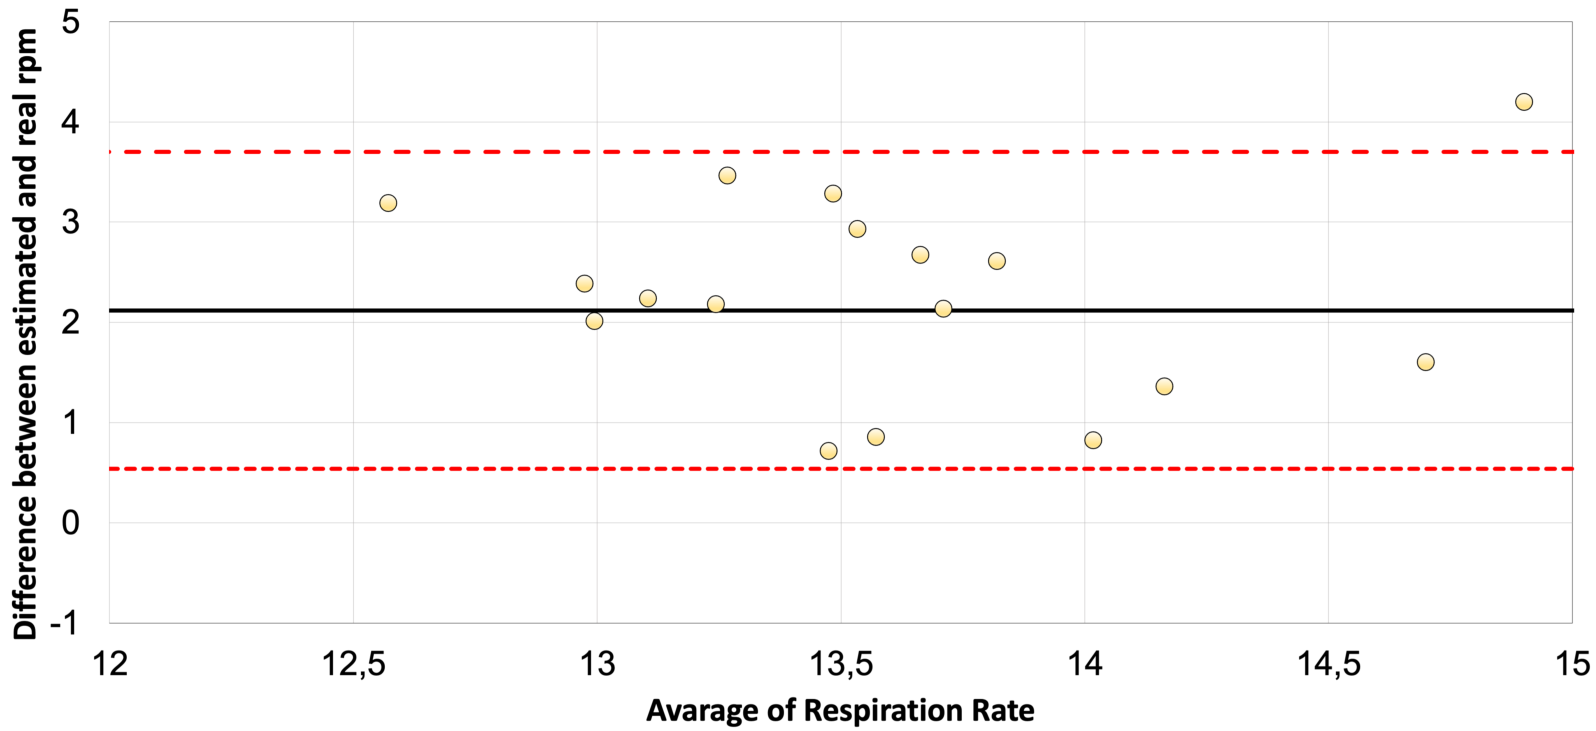
\includegraphics[width=\textwidth]{img/balnd1.pdf}
  \caption{Example of Bland Altman Plot}
  \label{fig:exxampleBland}
\end{figure}
\vspace{1cm}

The \textit{x-axis} of the plot displays the average measurement of the two instruments and the \textit{y-axis} displays the difference in measurements between the two instruments. In the plot are present also three lines, the central black represents the average difference in measurements between the two instruments also known as ``bias'' between the two measurements, as far from zero as large the average difference is large. The red dotted lines are the limits of the agreement, defined as the mean difference $\pm 1.96$ standard deviation of the difference. 




\clearpage
%%%%%% MODWTMRA %%%%%%
\section{Result for MODWTMRA} \label{cap:ResultMODWTRA}


This section of the result is divided into normal bed, section \ref{cap:ResultNormalBed1}, and rocking bed \ref{cap:ResultRockingBed1}. Inside both sections are presented the result for each position for the binary and weighted approach, the denoise method is MODWTMRA.

The estimated respiratory rate per minute (rpm) while the participants are on the mattressare further presented. Given the use of a moving window to simulate a real-time pipeline, the estimated rpm for each window is shown. 
The total number of windows for each position is 18 since the window is 60 seconds long and the entire recording for each position is 4 minutes long. 
First, is presented the table containing the estimated rpm using binary and weighted approaches compared with the rpm given by the ground truth. 
After is shown a table with the average rpm for both approaches and the relative mean absolute error (MAE) and mean absolute percentage error (MAPE). In the end, are presented the Bland–Altman plot to better visualize and understand the data in respect of the error and a plot of the best channel with its raw data and relative denoised wave.


%%%%%% NORMAL BED %%%%%%
\subsection{Normal Bed}

The participant in this phase has to perform a series of jumps before lying on the mattress due to recreating the increase or decrease of the breath rate between the different sleep stages. This phase aims to understand the feasibility of extracting breath rate from the mat. For this phase, the mattress is placed on a standard bed.

%%%%%% NORMAL BED - SUPINE %%%%%%

\subsubsection{Result Normal Bed in Supine Position}   \label{cap:ResultNormalBed1}

The estimated respiratory rate per minute (rpm) while the participants are supine with the mattress placed on a normal bed is further presented. Table \ref{tab:SupineNormalStill} presented the estimated rpm using binary and weighted approach compared with the rpm given by the ground truth. The approaches retrieve an almost identical rpm, this result may be due to the choice of the minimum confidence value at 80\% that allows keeping only the best signal, maybe with higher confidence can be seen a higher difference between the two approaches. 

\vspace{0.5cm}
\begin{table}[h]
    \centering
    \begin{tabular}{|c|c|c|}
    \hline 
     Binary  &  Weighted & RPM (NOXA1)  \\%& toolbox \\ 

    \hline 
     14.8438  & 14.7353  & 13.485 \\ % & 14 \\ %
   14  & 14  & 13.1443 \\%& 13 \\ 
     15.125  & 15.125 & 12.5154 \\ %& 13 \\ 
    13.8333  & 13.8333 &13.117\\ % & 13 \\ 
  14.4286  & 14.4286 & 13.6077\\ % & 14 \\ 
    15.5  & 15.5 & 13.8993\\ %& 15 \\ 
     15 &  15 & 12.0681\\ % & 15 \\ 
  11 &  11 & 11.4768\\ % & 15 \\ 
 14.3333 &  14.3333 & 12.1549 \\ %& 14 \\ 
  17 &  17 & 12.8028 \\ %& 13 \\ 
 15 &  15 & 12.3275 \\ %& 14 \\ 
 14.1667 & 14.1667 & 10.9785 \\ %& 11 \\ 
  15.125 & 15.125 & 11.8441 \\ %& 11 \\ 
 14.7778 &  14.7778 & 12.6438\\ % & 10 \\ 
    15 &  15 & 11.5351 \\ %& 11 \\ 
    14 & 14 & 11.99 \\ %& 10 \\ 
    14.2222 & 14.2222 & 11.9868 \\ %& 10 \\ 
    14.1667 &  13.8571 & 11.7824 \\ %& 10 \\ 

    \hline 
    \end{tabular}
    \caption{Estimated rpm using binary and weighted approach of the pipeline compared with the rpm given by the ground truth - Normal bed and supine position}
    \label{tab:SupineNormalStill}
\end{table}





 
    

Table \ref{tab:SupineNormalStillMetrics} present the average rpm for both approaches  
and the relative mean absolute error (MAE) and mean absolute percentage error (MAPE). As just discussed in the previous paragraph there is no substantial difference between the two different approaches. The data on which to focus more is the number of breaths that the algorithm misses, represented by MAE and expressed in percentage by MAPE. The average number is 2rpm, which means that if we consider the estimated average of 14.5rpm the error is almost 20\%, quite high for an approach that must be used in the medical field.

%\vspace{0.5cm}
\begin{table}[H]

    \centering
    \begin{tabular}{|c|c|c|}
    \hline 
    & Binary  & Weighted  \\ 
    \hline 
    rpm mean & 14.529 &  14.506\\
    MAE rpm  & 2.1731  &  2.1499 \\ 
    MAPE  & 17.8104\%  & 17.6198\% \\ 
    \hline 
    \end{tabular}
    
    \caption{Avarage number of breath for each approach with the relative mean absolute error (MAE) and mean absolute percentage error (MAE) - Normal bed and supine position}
    \label{tab:SupineNormalStillMetrics}
\end{table}

Figure \ref{fig:baln1} show the Bland–Altman plot, presented in section \ref{cap:plottino}, of the estimated rpm from the pipeline compared to the value of the ground truth. It helps to visualize the data from Table \ref{tab:SupineNormalStillMetrics} in respect of the error. Since the result for the approaches is similar the data presented with this plot refers to the weighted approach only.

Figure \ref{fig:rec} shows the denoised signal using MODWTMRA with the highest accuracy (92\%) for the supine position with a normal mattress.

\begin{figure}[p]
  \centering
  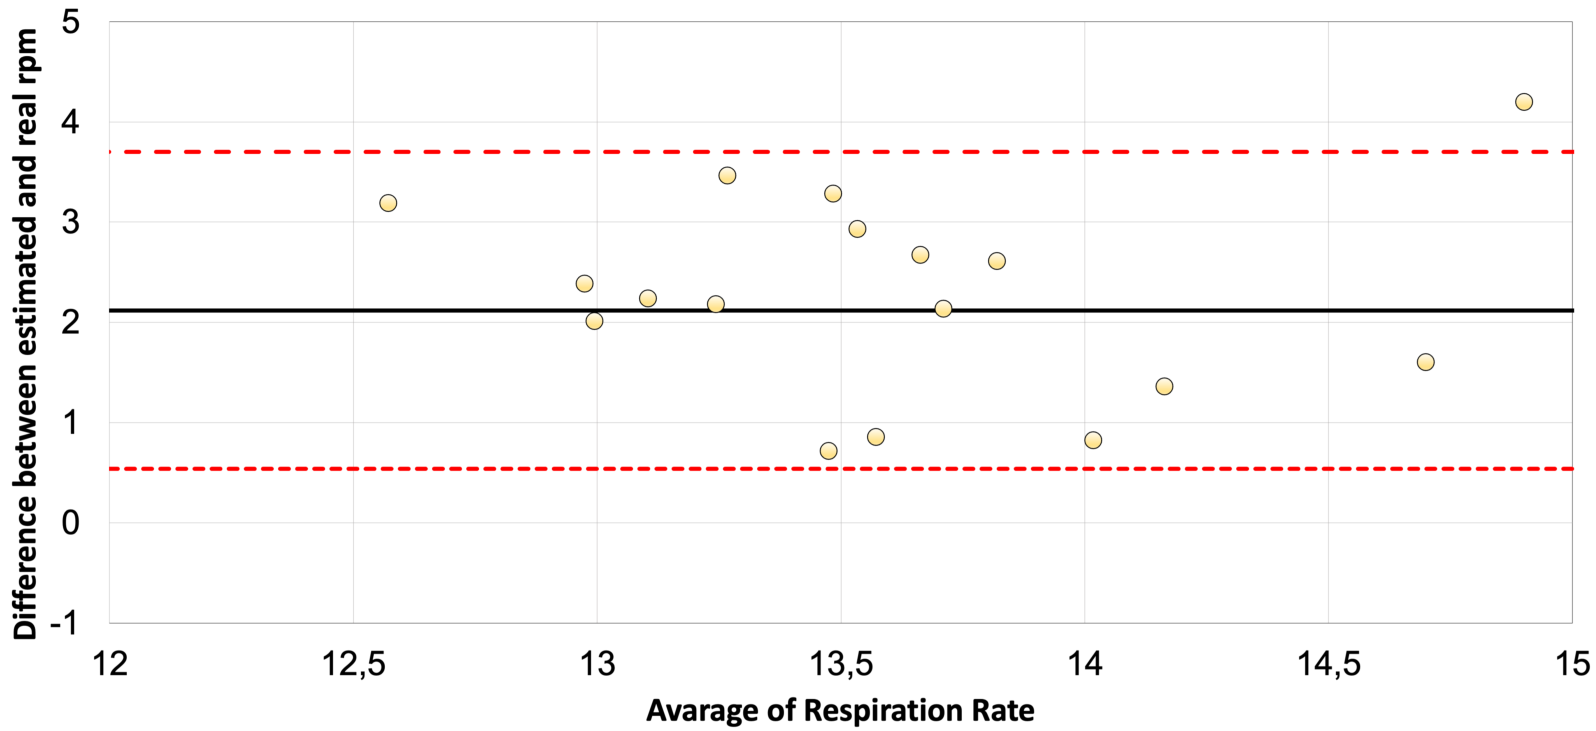
\includegraphics[width=\textwidth]{img/balnd1.pdf}

  \caption{Bland Altman Plot of estimated rpm from the pipeline compared to the value of the ground truth - Normal bed and supine position}
  \label{fig:baln1}
  \vspace{1.5cm}
  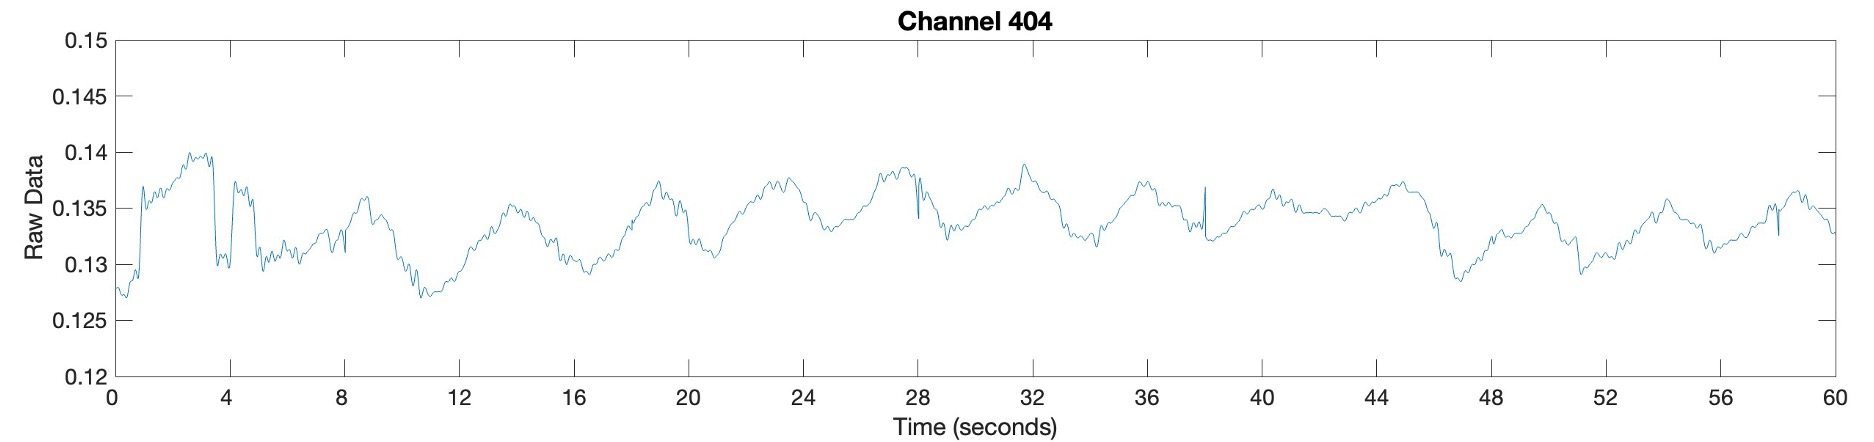
\includegraphics[width=\textwidth]{img/404.jpg}
  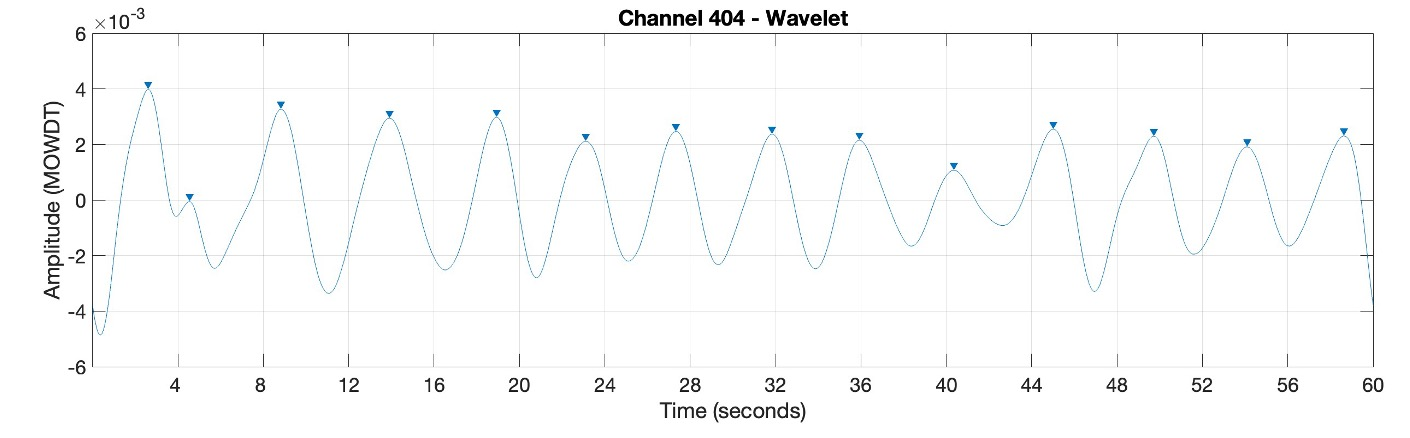
\includegraphics[width=\textwidth]{img/404_wave.jpg}
\caption{Raw data and denoised signal using MODWTMRA of the channel with the highest percentage of confidence (92\%) - Normal bed and supine position}
  \label{fig:rec}
\end{figure}


%%%%%% NORMAL BED - LEFT %%%%%%
\subsubsection{Result Normal Bed in Left Side Position}   \label{cap:ResultNormalBed2}

The estimated respiratory rate per minute (rpm) while the participants are on the left side with the mattress placed on a normal bed is further presented. Table \ref{tab:LeftNormalStill} presented the estimated rpm using binary and weighted approach compared with the rpm given by the ground truth. The approaches retrieve an almost identical rpm, this result may be due to the choice of the minimum confidence value at 80\% that allows keeping only the best signal, maybe with higher confidence can be seen a higher difference between the two approaches. 

\vspace{1.3cm}
%\begin{table}\begin{tabular}{|llllll|}
\hline 
Binary SGf & binary Waveleft & weighed  SGf & weighed Waveleft & resp rate & toolbox \\ 
\hline 
13.375 & 14.6364 & 13.375 & 14.6364 & 11.2045 & 10 \\ 
13.6667 & 15 & 13.6667 & 15 & 12.7397 & 11 \\ 
14 & 16 & 13.5 & 15.25 & 13.0613 & 12 \\ 
14.3571 & 14.2 & 14.3571 & 14.2 & 12.2669 & 12 \\ 
14 & 19 & 14 & 19 & 12.1628 & 13 \\ 
12.8 & 15 & 12.6667 & 14.5 & 13.6039 & 13 \\ 
11.8 & 14.2222 & 11.8 & 14.2222 & 13.1398 & 13 \\ 
14 & 15.6667 & 14 & 15.6667 & 11.5445 & 14 \\ 
13.8333 & 14.7 & 13.8333 & 14.7 & 10.77 & 11 \\ 
13.8889 & 15.8571 & 13.8889 & 15.8571 & 14.2216 & 12 \\ 
13.0833 & 15.5556 & 13.0833 & 15.5556 & 13.1656 & 12 \\ 
14.1111 & 16.5714 & 13.7 & 16.5714 & 12.9764 & 12 \\ 
14.2 & 15 & 14.2 & 15 & 10.9055 & 13 \\ 
13.25 & 15.125 & 13.25 & 15.125 & 13.2294 & 11 \\ 
12.7692 & 15.7143 & 12.2857 & 15.5 & 12.8524 & 11 \\ 
13.9167 & 15.2 & 13.6154 & 15.2 & 11.3824 & 13 \\ 
13 & 14.6 & 13 & 14.6 & 13.5579 & 11 \\ 
13 & 15.8889 & 13 & 15.8889 & 11.6069 & 12 \\ 
\hline 
\end{tabular}
\caption{Breath per minutes for each approach, result from Noxtural and toolbox
- Left position still mattress}
\end{table}

\begin{table}[h]
    \centering
    \begin{tabular}{|c|c|c|}
 
    \hline 
    Binary & Weighed &RPM (NOXA1) \\ 
    \hline 
   14.6364  & 14.6364 & 11.2045 \\ 
      15  & 15 & 12.7397 \\ 
      16  & 15.25 & 13.0613 \\  
  14.2  & 14.2 & 12.2669 \\ 
      19  & 19 & 12.1628 \\ 
      15  & 14.5 & 13.6039 \\ 
     14.2222  & 14.2222 & 13.1398 \\ 
     15.6667 & 15.6667 & 11.5445 \\ 
+ 14.7 & 14.7 & 10.77  \\ 
     15.8571  & 15.8571 & 14.2216 \\ 
 15.5556 & 15.5556 & 13.1656\\ 
 16.5714 & 16.5714 & 12.9764 \\ 
   15 &  15 & 10.9055 \\ 
15.125 & 15.125 & 13.2294 \\ 
15.7143& 15.5 & 12.8524 \\ 
     15.2 & 15.2 & 11.3824 \\ 
14.6 &  14.6 & 13.5579 \\ 
15.8889 & 15.8889 & 11.6069 \\ 
    \hline 
    \end{tabular}
    \caption{Estimated rpm using binary and weighted approach of the pipeline
    compared with the rpm given by the ground truth -
    - Normal bed and left side}
    \label{tab:LeftNormalStill}

\end{table}
    

\vspace{0.5cm}

Table \ref{tab:LeftNormalStillMetrics} present the average rpm for both approaches  
and the relative mean absolute error (MAE) and mean absolute percentage error (MAPE). As just discussed in the previous paragraph there is no substantial difference between the two different approaches. The data on which to focus more is the number of breaths that the algorithm misses, represented by MAE and expressed in percentage by MAPE. The average number is 2.5rpm, which means that if we consider the estimated average of 15.3rpm the error is over 24\%, worst than in the supine position, probably due to the smaller contact area between the body and the mattress.

\vspace{1cm}
\begin{table}[H]
    \centering

    \begin{tabular}{|c|c|c|}
    \hline 
    & Binary  & Weighed \\ 
    
    \hline 
    rpm mean & 15.441 & 15.360\\
    MAE resp  &   2.4545 &  2.8934 \\ 
    MAPE  & 24.62\% & 24.0041\% \\ 
    \hline 

    \end{tabular}
    \caption{varage number of breath for each approach with the relative mean
    absolute error (MAE) and mean absolute percentage error (MAE) - Normal bed
    and left side}
    \label{tab:LeftNormalStillMetrics}

    \end{table}
    
\vspace{0.5cm}

Figure \ref{fig:baln2} show the Bland–Altman plot, presented in section \ref{cap:plottino}, of the estimated rpm from the pipeline compared to the value of the ground truth. It helps to visualize the data from Table \ref{tab:LeftNormalStillMetrics} in respect of the error. Since the result for the approaches is similar the data presented with this plot refers to the weighted approach only.

Figure \ref{fig:rec} shows the denoised signal using MODWTMRA with the highest accuracy (92\%) for the supine position with a normal mattress.

\begin{figure}[p]
  \centering
  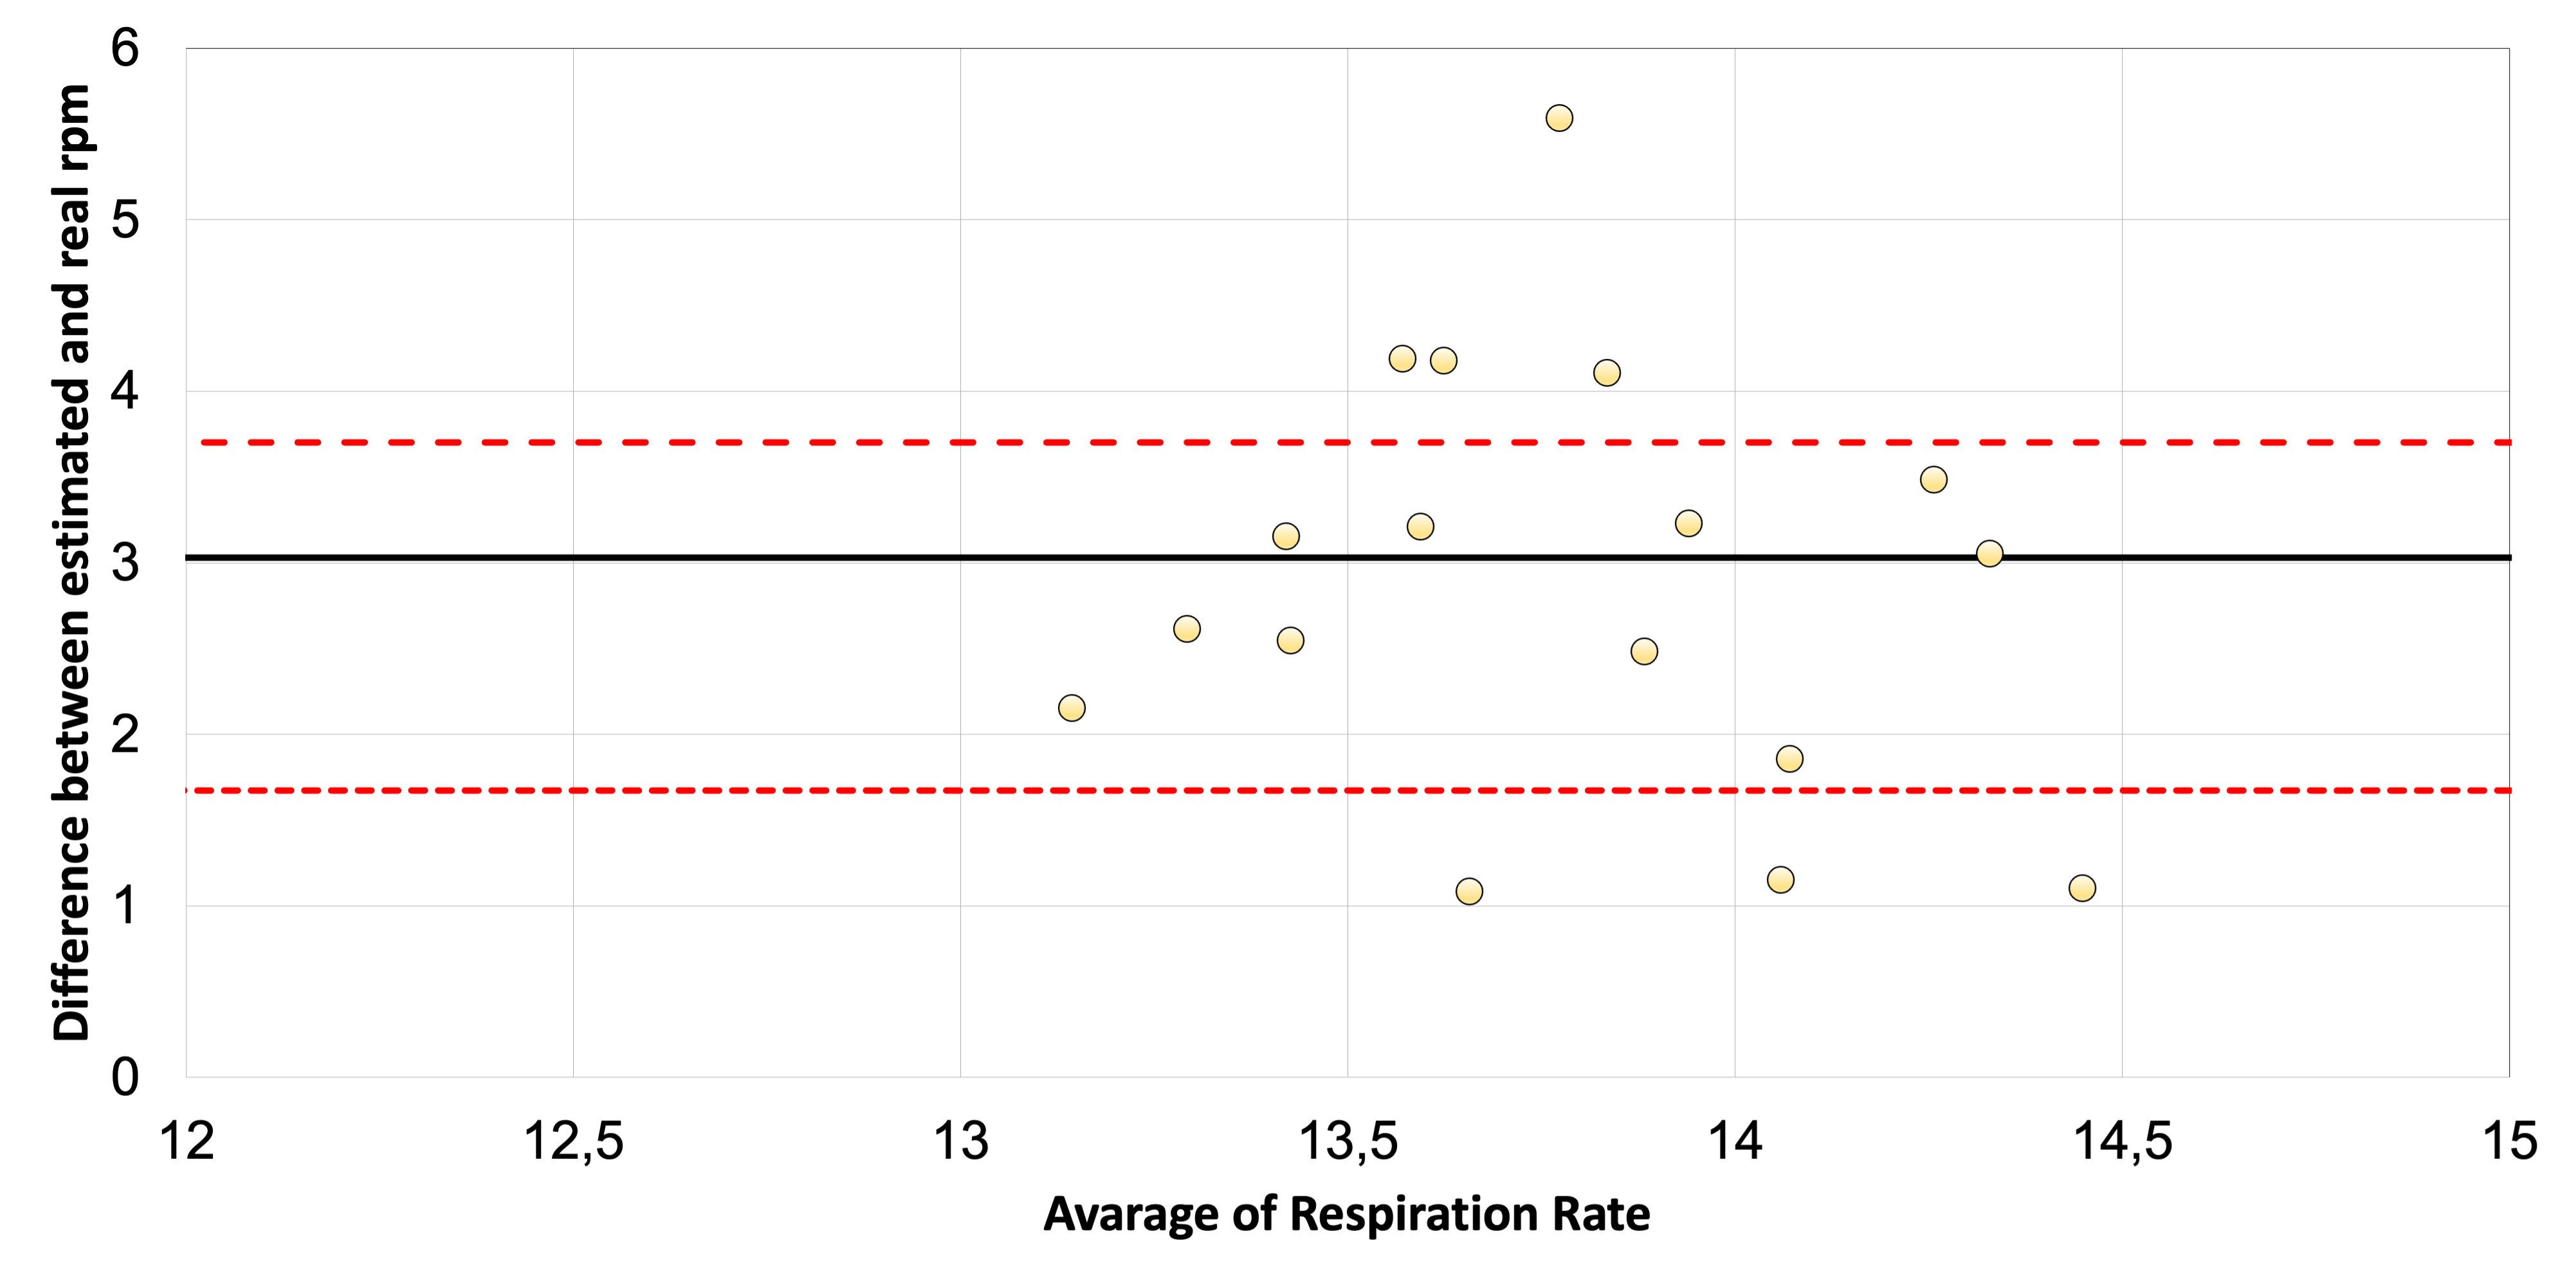
\includegraphics[width=\textwidth]{img/balnd2.png}

  \caption{Bland Altman Plot of estimated rpm from the pipeline compared to the value of the ground truth - Normal bed and left side}
  \label{fig:baln2}
  \vspace{1.5cm}
  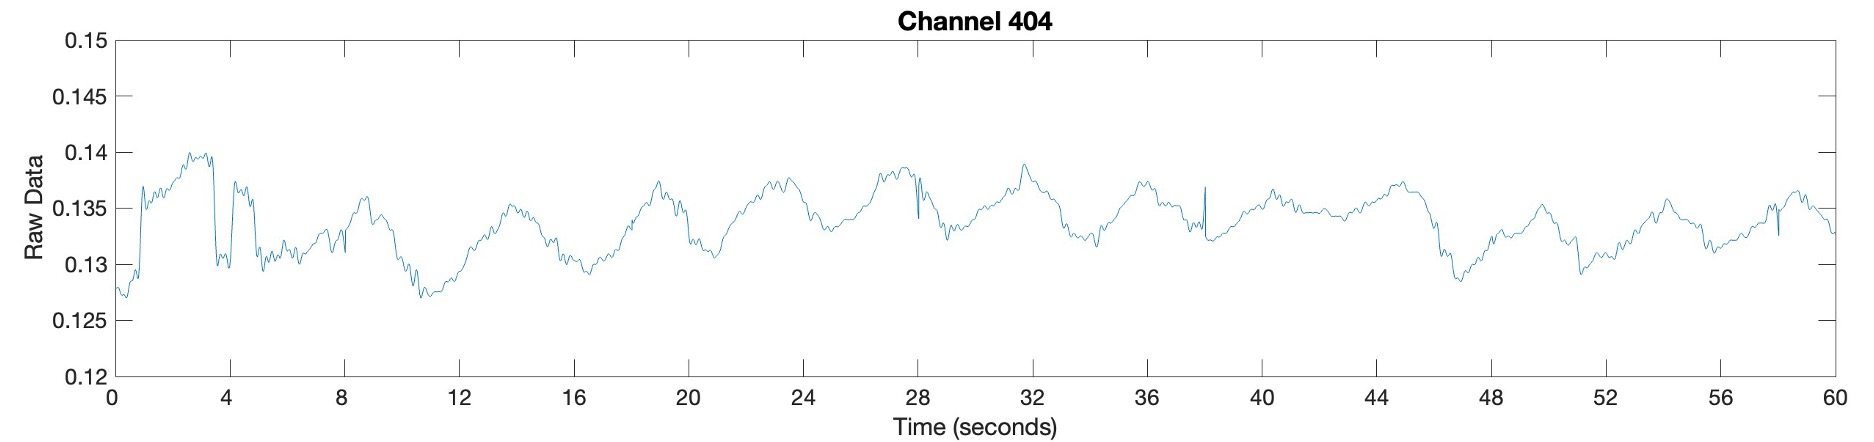
\includegraphics[width=\textwidth]{img/404.jpg}
  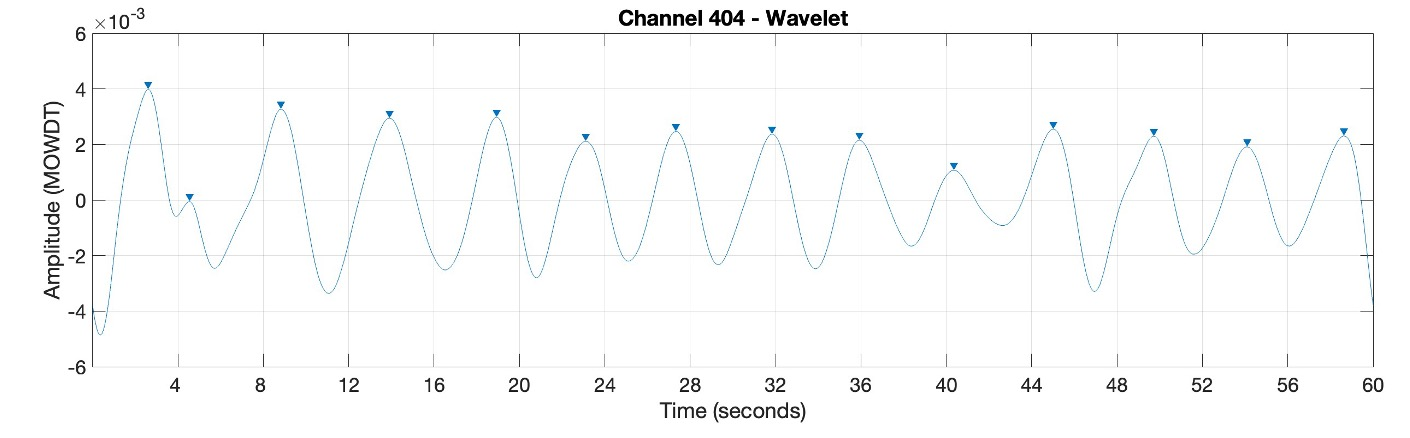
\includegraphics[width=\textwidth]{img/404_wave.jpg}
\caption{Raw data and denoised signal using MODWTMRA of the channel with the highest percentage of confidence (92\%) - Normal bed and supine position}
  \label{fig:rec}
\end{figure}


\clearpage
%%%%%% NORMAL BED - PRONE %%%%%%
\subsubsection{Result Normal Bed in Prone Side Position}   \label{cap:ResultNormalBed3}

The estimated respiratory rate per minute (rpm) while the participants are in the prone position with the mattress placed on a normal bed is further presented. Table \ref{tag:ProneNormalStill} presented the estimated rpm using binary and weighted approach compared with the rpm given by the ground truth. The approaches retrieve an almost identical rpm, this result may be due to the choice of the minimum confidence value at 80\% that allows keeping only the best signal, maybe with higher confidence can be seen a higher difference between the two approaches. 

\vspace{1.3cm}
%\begin{table}\begin{tabular}{|llllll|}
\hline 
Binary SGf & binary Waveleft & weighed  SGf & weighed Waveleft & resp rate & toolbox \\ 
\hline 
13.375 & 14.6364 & 13.375 & 14.6364 & 11.2045 & 10 \\ 
13.6667 & 15 & 13.6667 & 15 & 12.7397 & 11 \\ 
14 & 16 & 13.5 & 15.25 & 13.0613 & 12 \\ 
14.3571 & 14.2 & 14.3571 & 14.2 & 12.2669 & 12 \\ 
14 & 19 & 14 & 19 & 12.1628 & 13 \\ 
12.8 & 15 & 12.6667 & 14.5 & 13.6039 & 13 \\ 
11.8 & 14.2222 & 11.8 & 14.2222 & 13.1398 & 13 \\ 
14 & 15.6667 & 14 & 15.6667 & 11.5445 & 14 \\ 
13.8333 & 14.7 & 13.8333 & 14.7 & 10.77 & 11 \\ 
13.8889 & 15.8571 & 13.8889 & 15.8571 & 14.2216 & 12 \\ 
13.0833 & 15.5556 & 13.0833 & 15.5556 & 13.1656 & 12 \\ 
14.1111 & 16.5714 & 13.7 & 16.5714 & 12.9764 & 12 \\ 
14.2 & 15 & 14.2 & 15 & 10.9055 & 13 \\ 
13.25 & 15.125 & 13.25 & 15.125 & 13.2294 & 11 \\ 
12.7692 & 15.7143 & 12.2857 & 15.5 & 12.8524 & 11 \\ 
13.9167 & 15.2 & 13.6154 & 15.2 & 11.3824 & 13 \\ 
13 & 14.6 & 13 & 14.6 & 13.5579 & 11 \\ 
13 & 15.8889 & 13 & 15.8889 & 11.6069 & 12 \\ 
\hline 
\end{tabular}
\caption{Breath per minutes for each approach, result from Noxtural and toolbox
- Left position still mattress}
\end{table}

\begin{table}[h]
    \centering
    \begin{tabular}{|c|c|c|}
    \hline 
    Binary & Weighed  SGf & RPM (NOXA1) \\ 
    \hline 
     15.7 & 15.7 & 11.5949 \\ 
    15.7333  & 15.7333 & 11.1628\\ 
   16.1  & 16.1 & 11.0005 \\ 
     15.6667 & 15.6667 & 10.4762  \\ 
  15.25  & 15.25 & 10.4723 \\ 
     14.5714 & 14.5714 & 9.5345  \\ 
     15.5714  & 15.5714 & 9.5467 \\ 
    15.875& 15.875 & 13.5758  \\ 
 14  & 14 & 11.1779  \\ 
     14.375  & 14.375 & 9.5345  \\ 
      14.4667  & 14.4667 & 9.5841 \\ 
 14.5  & 14.5 & 11.8196  \\ 
 14.2143 & 14.2143 & 11.8153  \\ 
 13.9474  & 13.9474 & 9.5223  \\ 
   15.037  & 15.037 & 10.8508  \\ 
 14.931  & 14.931 & 10.8876  \\ 
     15.25  & 15.25 & 10.9705  \\ 
     15.3333 & 15.3333 & 11.237  \\ 
    \hline 
    \end{tabular}
    
    \caption{Estimated rpm using binary and weighted approach of the pipeline
    compared with the rpm given by the ground truth - Normal bed and supine position}
    \label{tag:ProneNormalStill}
    \end{table}
    
    

\vspace{0.5cm}

Table \ref{tab:ProneNormalStillMetrics} present the average rpm for both approaches  
and the relative mean absolute error (MAE) and mean absolute percentage error (MAPE). As just discussed in the previous paragraph there is no substantial difference between the two different approaches. The data on which to focus more is the number of breaths that the algorithm misses, represented by MAE and expressed in percentage by MAPE. The average number is 2.8rpm, which means that if we consider the estimated average of 15rpm the error is over 36\%, worst worse than the two previous results it may depend on the movement of the chest in the prone position changes.


\vspace{1cm}
\begin{table}[H]
    \centering
    \begin{tabular}{|c|c|c|}
    \hline 
    & Binary & Weighed \\ 
    
    \hline 

    rpm mean   &  15.029 &  15.029 \\
    MAE rpm & 2.8957 \% &  2.8957\% \\
    MAPE tool  & 36.5982 & 36.5982 \\ 
    \hline 
    \end{tabular}
    
    \caption{Metrics to evaluate the participant in belly position with moving mattress}
    \label{tab:ProneNormalStillMetrics}
    \end{table}
    
\vspace{0.5cm}

Figure \ref{fig:baln2} show the Bland–Altman plot, presented in section \ref{cap:plottino}, of the estimated rpm from the pipeline compared to the value of the ground truth. It helps to visualize the data from Table \ref{tab:ProneNormalStillMetrics} in respect of the error. Since the result for the approaches is similar the data presented with this plot refers to the weighted approach only.

Figure \ref{fig:rec} shows the denoised signal using MODWTMRA with the highest accuracy (92\%) for the supine position with a normal mattress.

\begin{figure}[p]
  \centering
  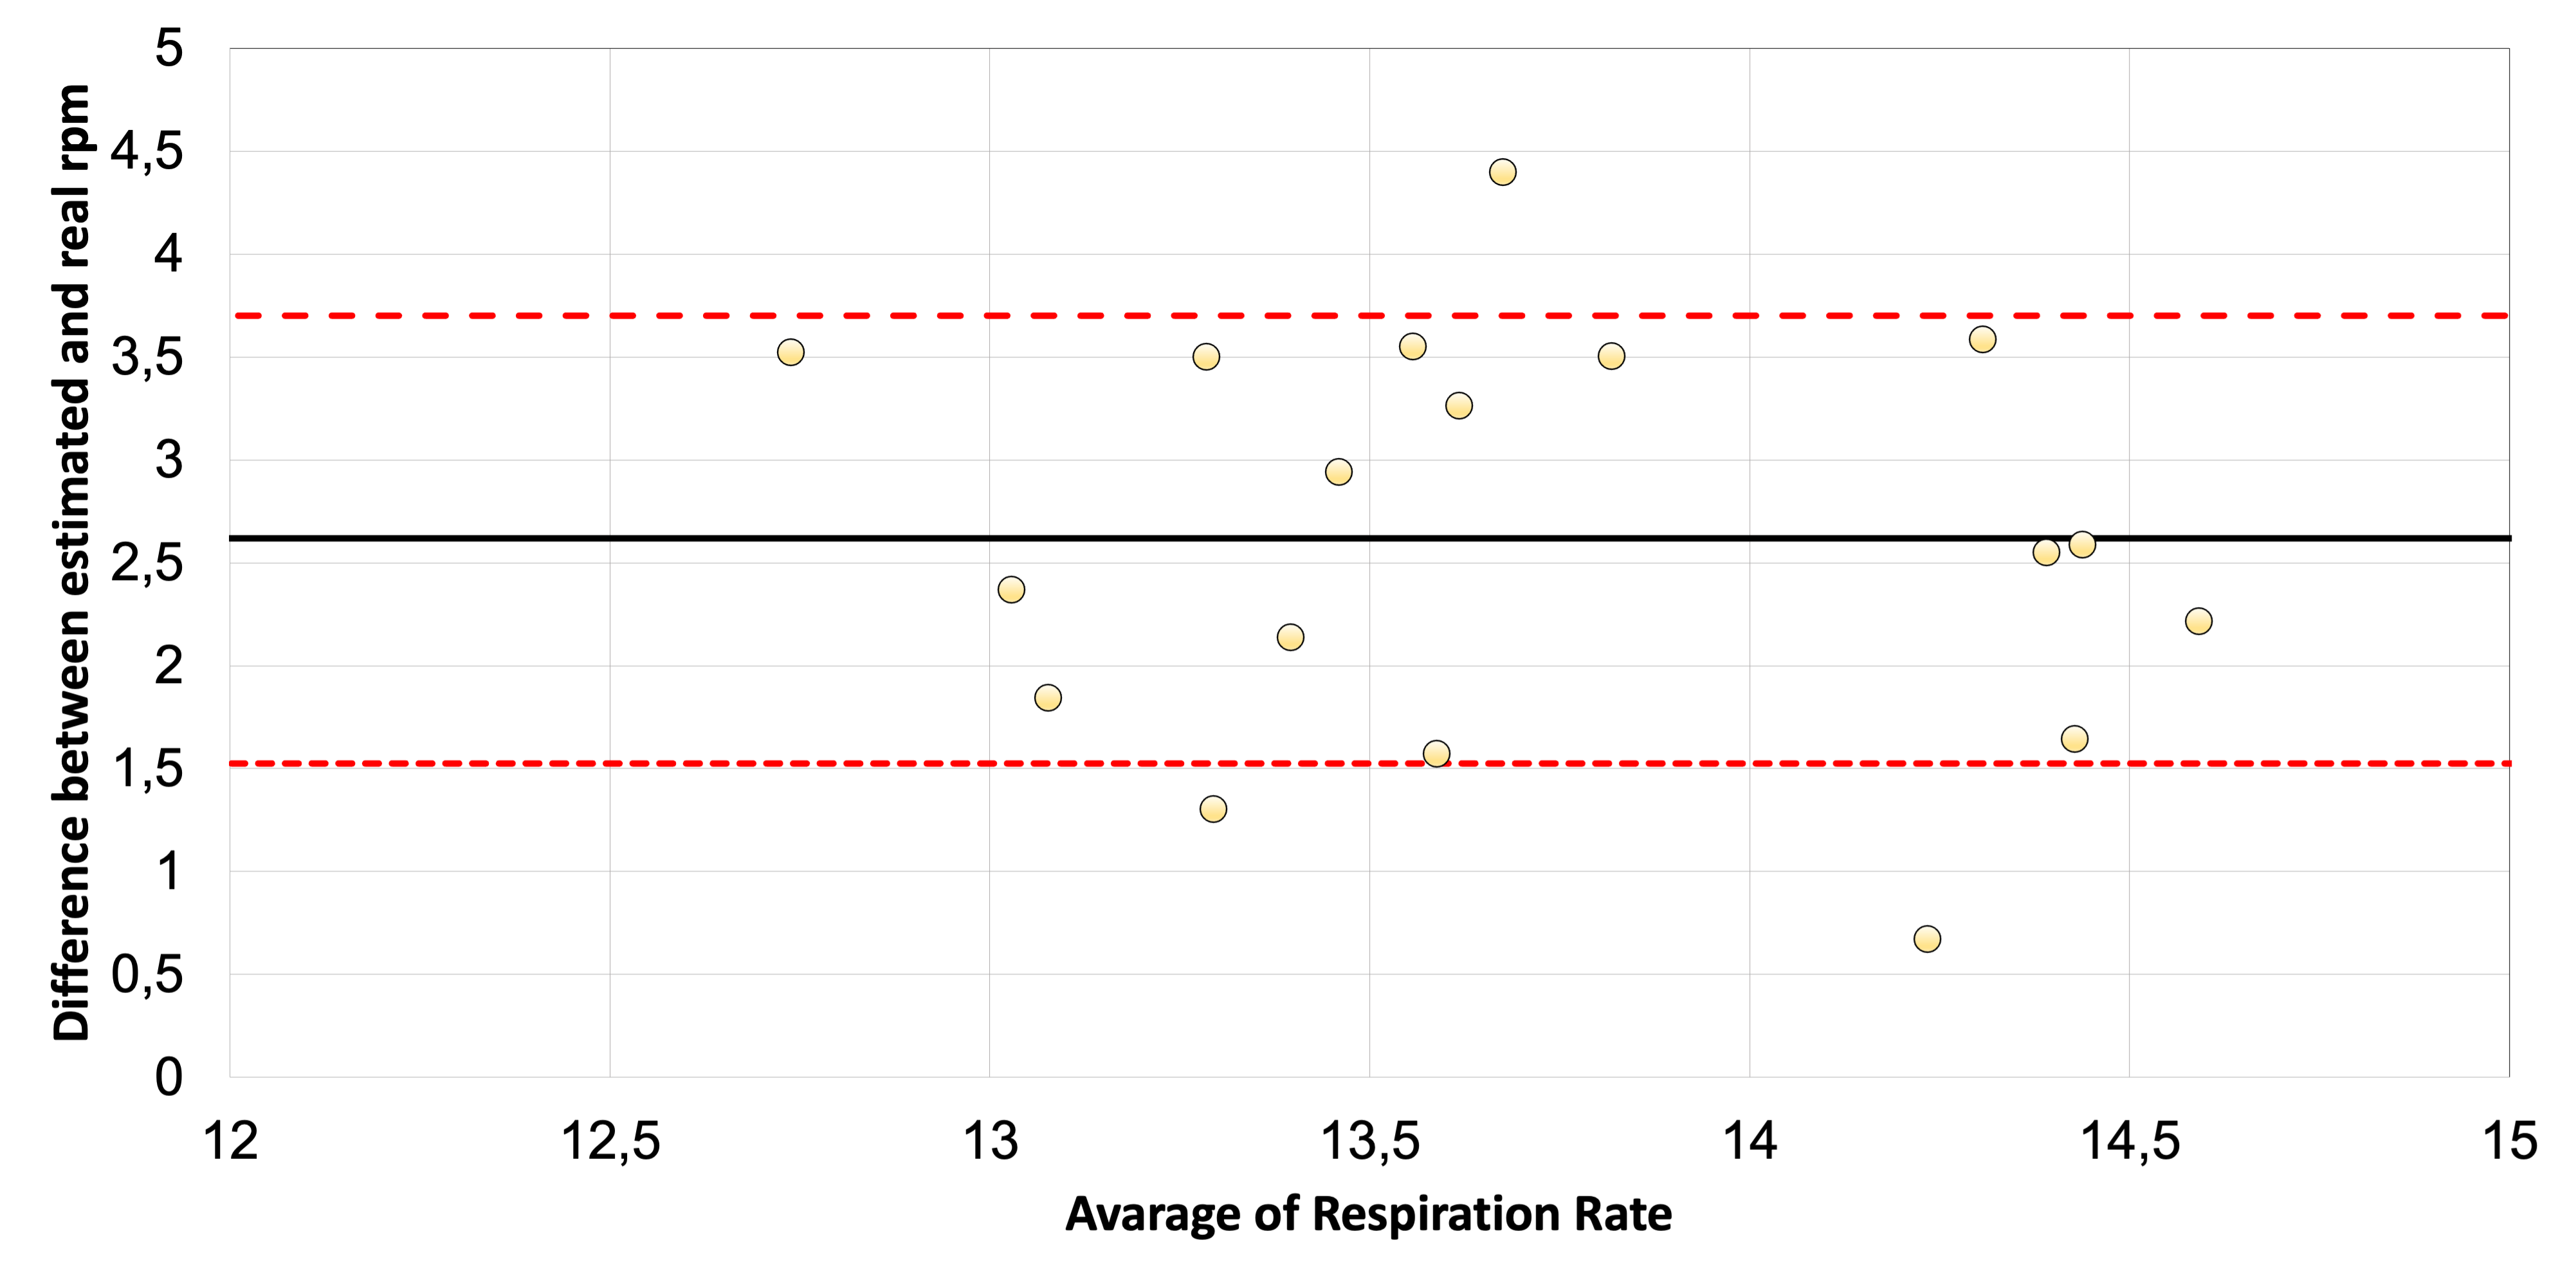
\includegraphics[width=\textwidth]{img/balnd3.png}

  \caption{Bland Altman Plot of estimated rpm from the pipeline compared to the value of the ground truth - Normal bed and prone position}
  \label{fig:baln2}
  \vspace{1.5cm}
  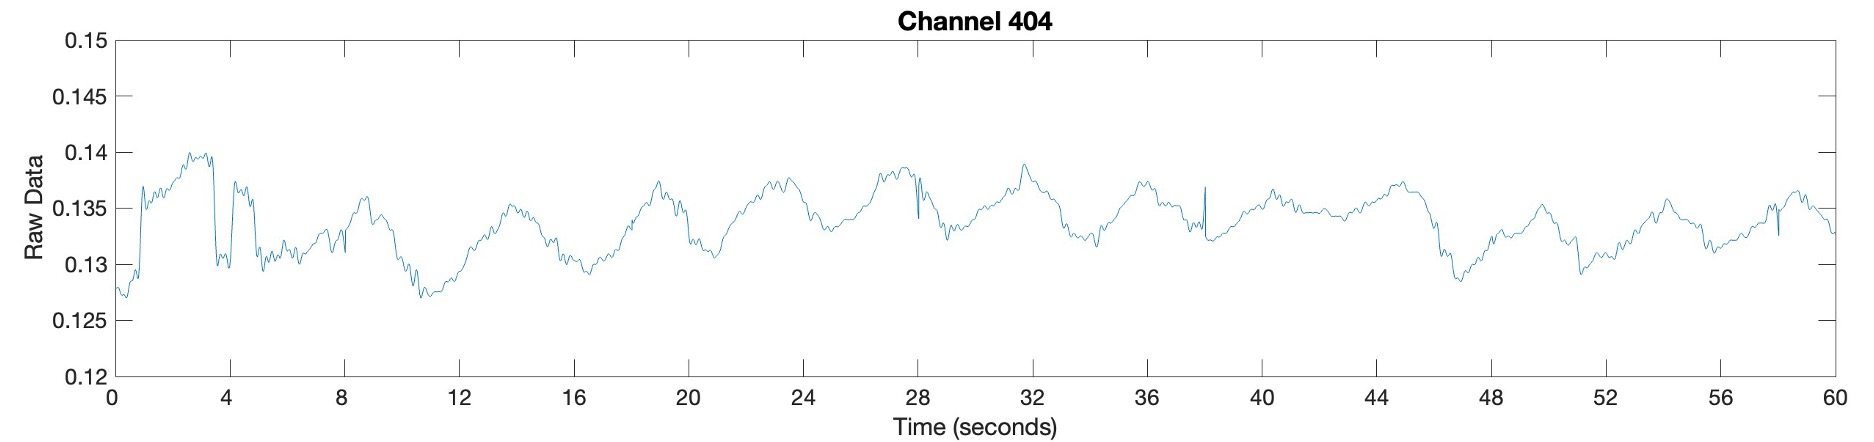
\includegraphics[width=\textwidth]{img/404.jpg}
  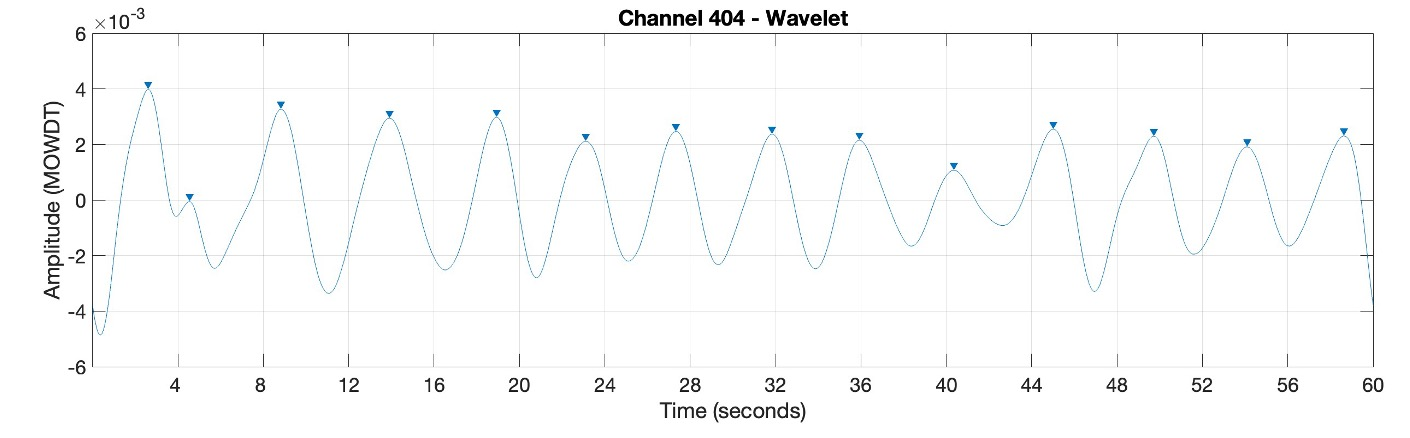
\includegraphics[width=\textwidth]{img/404_wave.jpg}
\caption{Raw data and denoised signal using MODWTMRA of the channel with the highest percentage of confidence (92\%) - Normal bed and supine position}
  \label{fig:rec}
\end{figure}

\clearpage
%%%%%% NORMAL BED - RIGHT %%%%%%
\subsubsection{Result Normal Bed in Right Side Position}   \label{cap:ResultNormalBed4}

The estimated respiratory rate per minute (rpm) while the participants are on the right side with the mattress placed on a normal bed is further presented. Table \ref{tab:RightNormalStill} presented the estimated rpm using binary and weighted approach compared with the rpm given by the ground truth. The approaches retrieve an almost identical rpm, this result may be due to the choice of the minimum confidence value at 80\% that allows keeping only the best signal, maybe with higher confidence can be seen a higher difference between the two approaches. 

\vspace{1cm}
%\begin{table}\begin{tabular}{|llllll|}
\hline 
Binary SGf & binary Waveleft & weighed  SGf & weighed Waveleft & resp rate & toolbox \\ 
\hline 
13.375 & 14.6364 & 13.375 & 14.6364 & 11.2045 & 10 \\ 
13.6667 & 15 & 13.6667 & 15 & 12.7397 & 11 \\ 
14 & 16 & 13.5 & 15.25 & 13.0613 & 12 \\ 
14.3571 & 14.2 & 14.3571 & 14.2 & 12.2669 & 12 \\ 
14 & 19 & 14 & 19 & 12.1628 & 13 \\ 
12.8 & 15 & 12.6667 & 14.5 & 13.6039 & 13 \\ 
11.8 & 14.2222 & 11.8 & 14.2222 & 13.1398 & 13 \\ 
14 & 15.6667 & 14 & 15.6667 & 11.5445 & 14 \\ 
13.8333 & 14.7 & 13.8333 & 14.7 & 10.77 & 11 \\ 
13.8889 & 15.8571 & 13.8889 & 15.8571 & 14.2216 & 12 \\ 
13.0833 & 15.5556 & 13.0833 & 15.5556 & 13.1656 & 12 \\ 
14.1111 & 16.5714 & 13.7 & 16.5714 & 12.9764 & 12 \\ 
14.2 & 15 & 14.2 & 15 & 10.9055 & 13 \\ 
13.25 & 15.125 & 13.25 & 15.125 & 13.2294 & 11 \\ 
12.7692 & 15.7143 & 12.2857 & 15.5 & 12.8524 & 11 \\ 
13.9167 & 15.2 & 13.6154 & 15.2 & 11.3824 & 13 \\ 
13 & 14.6 & 13 & 14.6 & 13.5579 & 11 \\ 
13 & 15.8889 & 13 & 15.8889 & 11.6069 & 12 \\ 
\hline 
\end{tabular}
\caption{Breath per minutes for each approach, result from Noxtural and toolbox
- Left position still mattress}
\end{table}


\begin{table}[H]
    \centering
    \begin{tabular}{|c|c|c|}
    \hline 
    Binary & Weighed  & RPM (NOXA1) \\ 
    
    \hline 
     16.1667   & 16.1667 & 12.4771 \\ 
     17.75  & 17.75 & 13.0835 \\ 
      16.5   & 16.5 & 14.3858 \\  
     15.25   & 15.25 & 12.7261 \\ 
  15.8333   & 15.8333 & 13.4867 \\ 
     15   & 15 & 12.9816 \\ 
     15.2353 &   15.2353 & 14.0566 \\ 
      15.1667  & 15.1667 & 12.038 \\ 
     15.5  & 15.5 & 11.4923 \\ 
     13  & 13 & 11.9625 \\ 
     13.3333   & 13.5 & 11.0151 \\ 
      15.5   & 15.5 & 11.9016 \\ 
     14.3333  & 14.3333 & 11.4255 \\ 
   13.8333  & 13.8333 & 12.5227 \\  
     15.2   & 15.2 & 11.5945 \\ 
      14.0909   & 14.0909 & 13.4141 \\  
     14.5   & 14.4286 & 13.5282 \\ 
      15.2308   & 15.2308 & 12.9839 \\ 
    \hline 
    \end{tabular}
    \caption{Estimated rpm using binary and weighted approach of the pipeline
    compared with the rpm given by the ground truth - Normal bed and right side}
    \label{tab:RightNormalStill}
    \end{table}

\vspace{0.5cm}

Table \ref{tab:RightNormalStillMetrics} present the average rpm for both approaches  
and the relative mean absolute error (MAE) and mean absolute percentage error (MAPE). As just discussed in the previous paragraphs there is no substantial difference between the two different approaches. The data on which to focus more is the number of breaths that the algorithm misses, represented by MAE and expressed in percentage by MAPE. The average number is 2.5rpm, which means that if we consider the estimated average of 15rpm the error is almost 20\%, worst than in the supine position but better than in the prone position and left side.

\vspace{1cm}
\begin{table}[H]
    \centering
    \begin{tabular}{|c|c|c|}
    \hline 
    & Binary  & Weighed \\ 
    \hline 
    rpm mean & 15.015 & 15.020\\
    MAE resp &  2.4638  &  2.4691  \\ 
    MAPE  &  19.9146 \%&  19.9693 \%\\ 
    \hline 
    \end{tabular}
    
    \caption{Evarage number of breath for each approach with the relative mean
    absolute error (MAE) and mean absolute percentage error (MAE) - Normal bed
    and right side}
    \label{tab:RightNormalStillMetrics}
    \end{table}
    
\vspace{0.5cm}

Figure \ref{fig:baln4} show the Bland–Altman plot, presented in section \ref{cap:plottino}, of the estimated rpm from the pipeline compared to the value of the ground truth. It helps to visualize the data from Table \ref{tab:RightNormalStillMetrics} in respect of the error. Since the result for the approaches is similar the data presented with this plot refers to the weighted approach only.

Figure \ref{fig:rec4} shows the denoised signal using MODWTMRA with the highest accuracy (92\%) for the supine position with a normal mattress.

\begin{figure}[p]
  \centering
  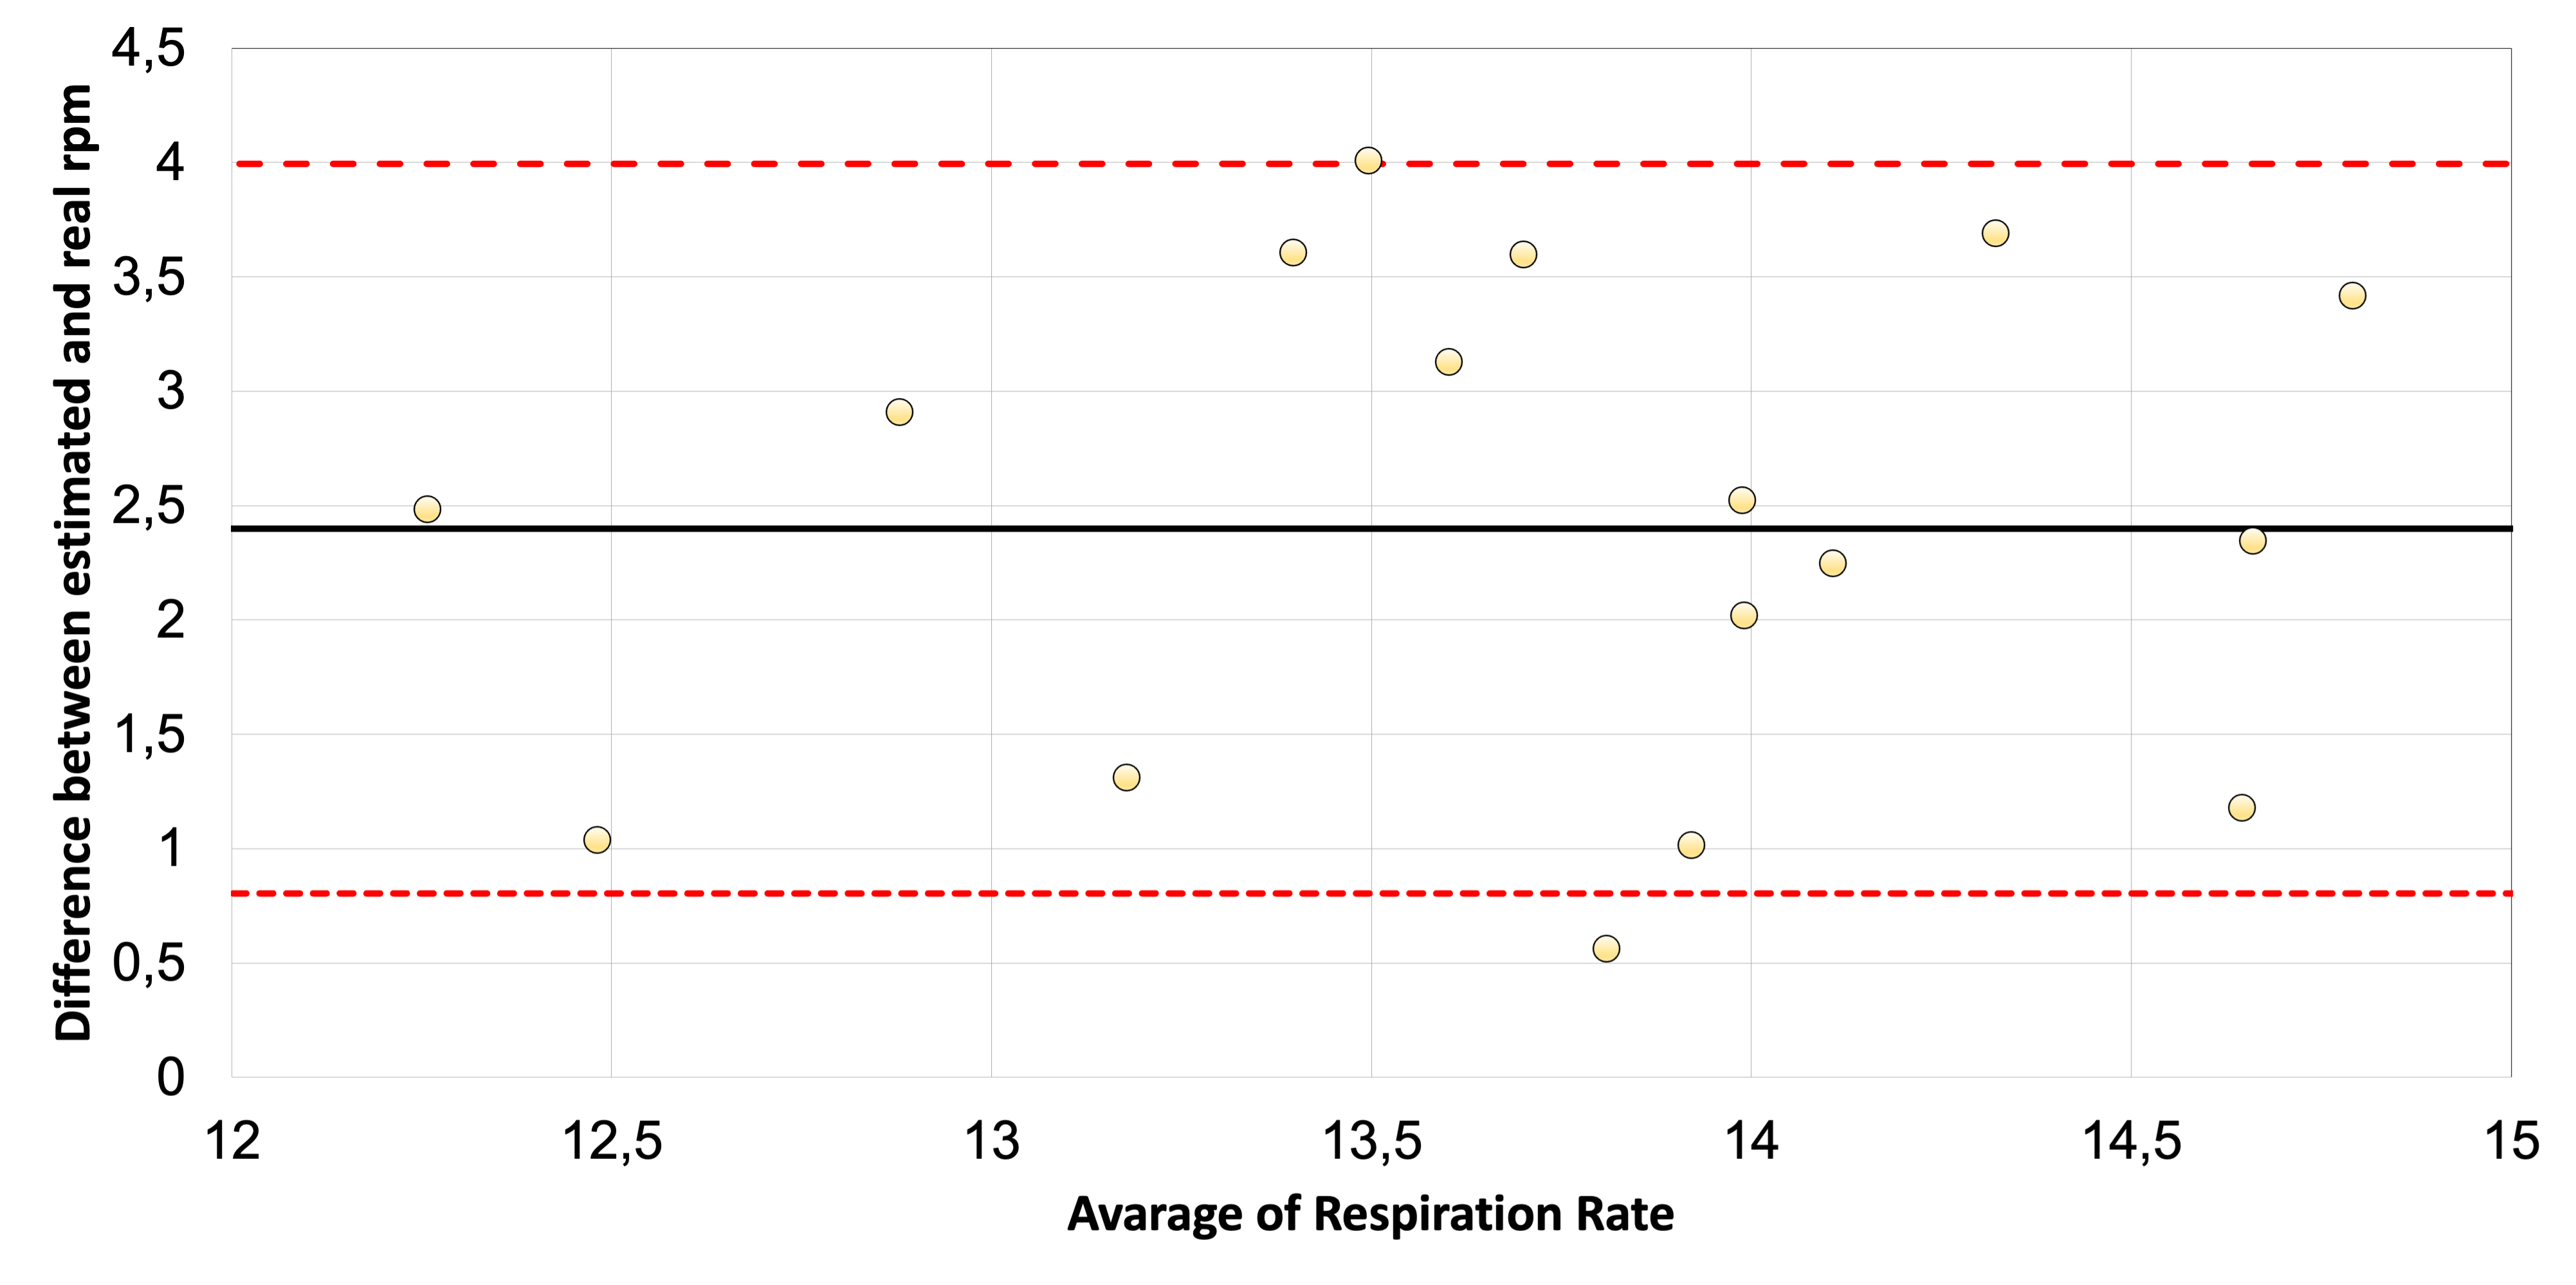
\includegraphics[width=\textwidth]{img/balnd4.png}

  \caption{Bland Altman Plot of estimated rpm from the pipeline compared to the value of the ground truth - Normal bed and left side}
  \label{fig:baln4}
  \vspace{1.5cm}
  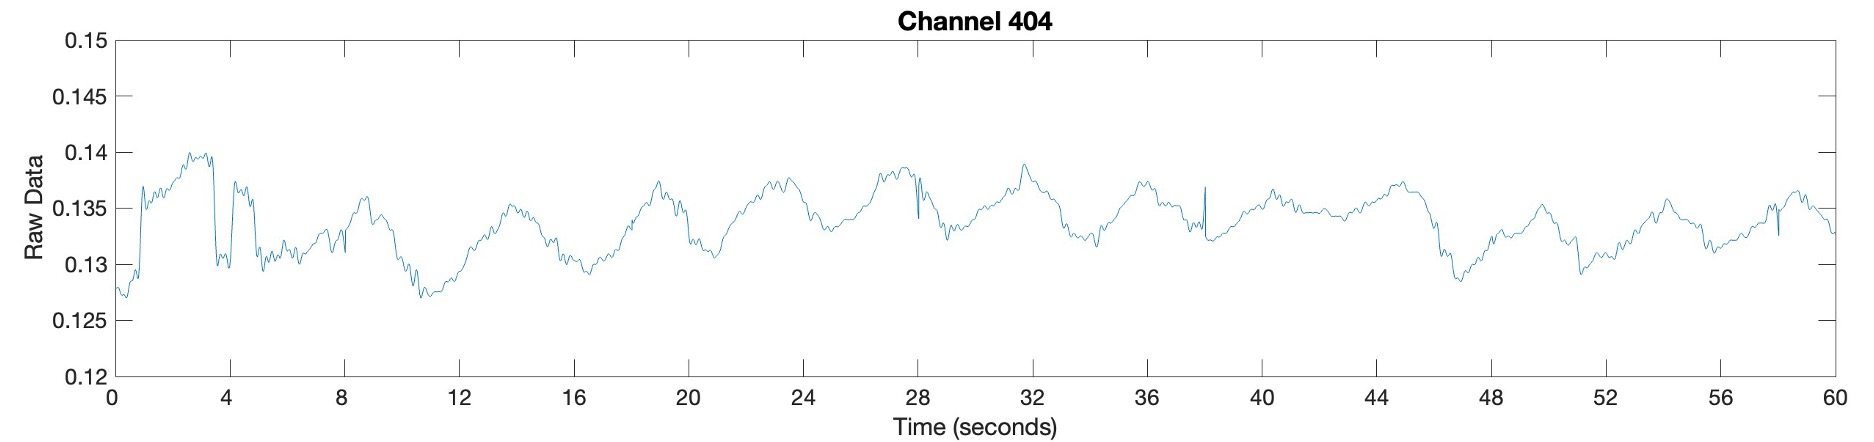
\includegraphics[width=\textwidth]{img/404.jpg}
  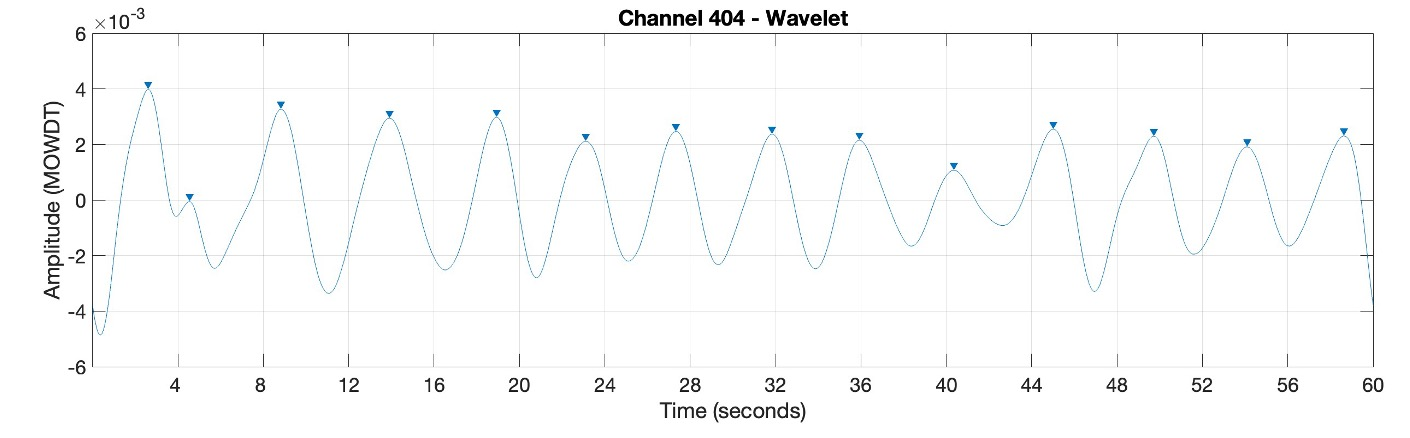
\includegraphics[width=\textwidth]{img/404_wave.jpg}
\caption{Raw data and denoised signal using MODWTMRA of the channel with the highest percentage of confidence (92\%) - Normal bed and supine position}
  \label{fig:rec4}
\end{figure}

\clearpage
%%%%%% Rocking  Bed %%%%%%
\subsection{Rocking Bed}
The second part of the data collection aims to understand if the movement of the
rocking bed could influence the signal. The participant has to lie on the mattress without jumps, to have less variability in the data. For this phase, the mattress is placed on a rocking bed, which periods have been fixed at 4 seconds (15 periods in a minute) with an acceleration of 0.25 $m/s^2$.


%%%%%% Rocking BED - SUPINE %%%%%%

\subsubsection{Result Rocking Bed in Supine Position}  % \label{cap:ResultNormalBed1}

The estimated respiratory rate per minute (rpm) while the participants are supine with the mattress placed on a rocking bed is further presented. 

Table \ref{tab:SupineMov} presented the estimated rpm using binary and weighted approach compared with the rpm given by the ground truth. The approaches retrieve an almost identical rpm. 

\vspace{0.5cm}
\begin{table}[H]
    \centering
    \begin{tabular}{|c|c|c|}
    \hline 
    Binary & Weighed  & RPM (NOXA1) \\ 
    \hline
15.5       &  15.5    &  10.7609 \\ 
16.1333     & 16.1333  &    11.3077 \\ 
15.3333    &  15.3333   &   13.1449 \\ 
14.9474    &  14.9474    &  11.3366 \\ 
15.1       &  15.1     & 12.7314 \\ 
15.6364   &   15.6364   &   11.8892 \\ 
14.6923    &  14.6923    &    11.42 \\ 
15.2222    &  15.2222    &  13.0092 \\ 
15.1667    &  15.1667    &  13.2539 \\ 
14.6667    &  14.6667    &  11.6391 \\ 
15         &  15    &  12.2165 \\ 
14.75       & 14.75  &    11.9216 \\ 
15           &15    &  11.3091 \\ 
14.625    &   14.625   &   13.8905 \\ 
15.6154    &  15.6154   &   11.3344 \\ 
15   &   14.8182   &   11.4474 \\ 
15.1765   &   15.1765   &   11.6675 \\ 
14.6154  &    14.6154    &  13.4799 \\
\hline 
    \end{tabular}
\caption{Estimated rpm using binary and weighted approach of the pipeline compared with the rpm given by the ground truth - Rocking bed and supine position}
\label{tab:SupineMov}
\end{table}

Table \ref{tab:SupineMov} present the average rpm for both approaches  
and the relative mean absolute error (MAE) and mean absolute percentage error (MAPE). As just discussed in the previous paragraph there is no substantial difference between the two different approaches. The data on which to focus more is the number of breaths that the algorithm misses, represented by MAE and expressed in percentage by MAPE. The average number is 3rpm, which means that if we consider the estimated average of 15.1rpm the error is almost 25\%, is too high for an approach that must be used in the medical field.

%\vspace{0.5cm}

\begin{table}[h]

    \centering

\begin{tabular}{|c|c|c|c|c|}
\hline 
& Binary & Weighed \\ 
 
\hline 
rpm mean & 15.1211  & 15.1110 \\  
MAE resp   & 3.0234 &     3.0133 \\ 
MAPE resp  & 25.7324\% &  25.6442\% \\ 

\hline 
\end{tabular}
\caption{Evarage number of breath for each approach with the relative mean
absolute error (MAE) and mean absolute percentage error (MAE) - Rocking bed
and right side}
\label{tab:SupineRockingMetrics}
\end{table}

Figure \ref{fig:baln1} show the Bland–Altman plot, presented in section \ref{cap:plottino}, of the estimated rpm from the pipeline compared to the value of the ground truth. It helps to visualize the data from Table \ref{tab:SupineRockingMetrics} in respect of the error. Since the result for the approaches is similar the data presented with this plot refers to the weighted approach only.

Figure \ref{fig:rec} shows the denoised signal using MODWTMRA with the highest accuracy (92\%) for the supine position with a normal mattress.

\begin{figure}[p]
  \centering
  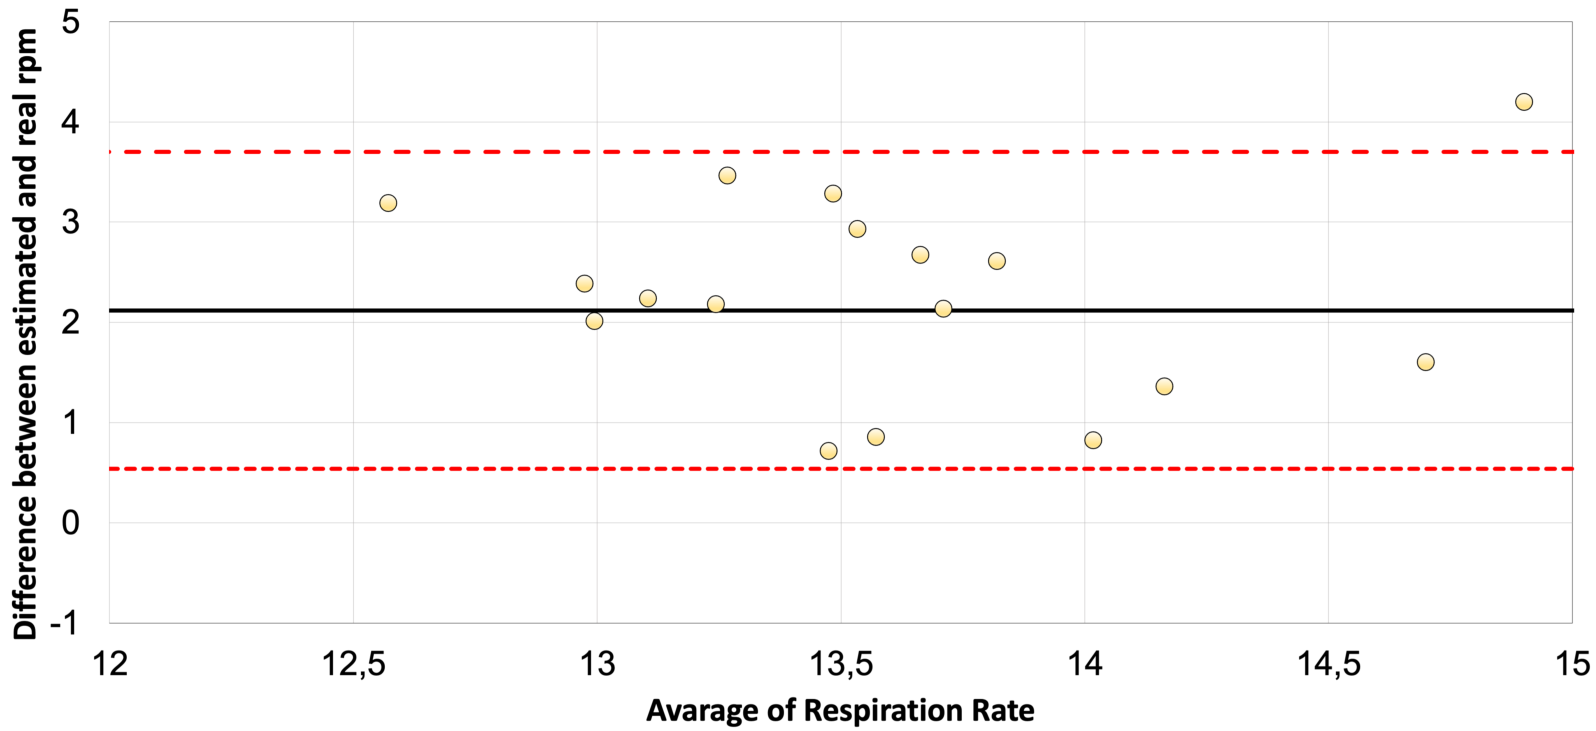
\includegraphics[width=\textwidth]{img/balnd1.pdf}

  \caption{Bland Altman Plot of estimated rpm from the pipeline compared to the value of the ground truth - Rocking bed and supine position}
  \label{fig:baln1}
  \vspace{1.5cm}
  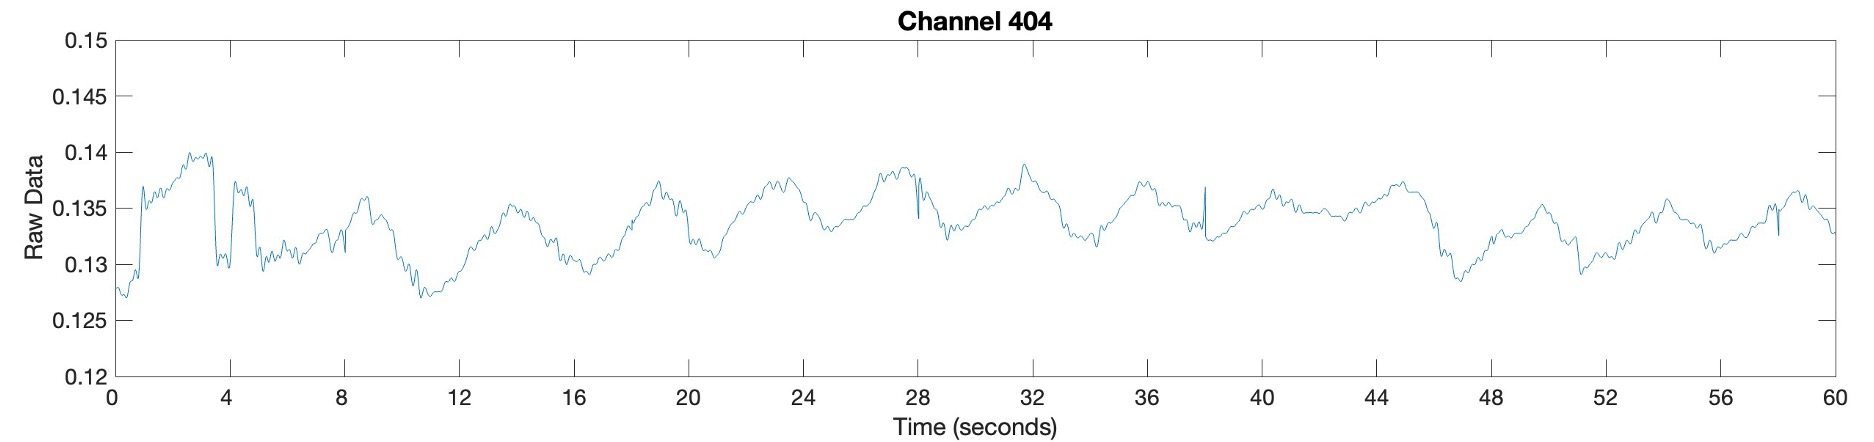
\includegraphics[width=\textwidth]{img/404.jpg}
  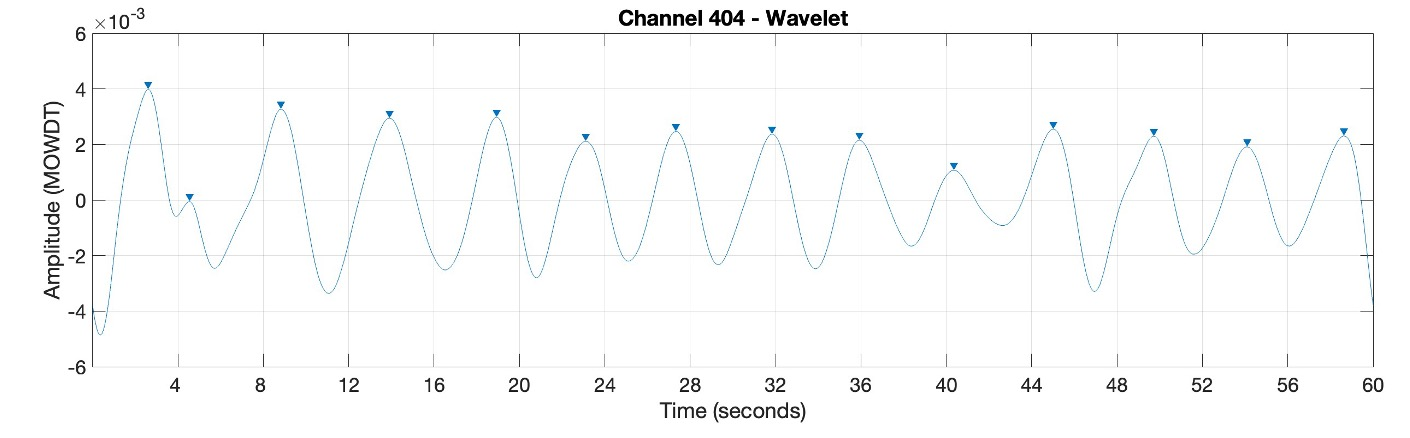
\includegraphics[width=\textwidth]{img/404_wave.jpg}
\caption{Raw data and denoised signal using MODWTMRA of the channel with the highest percentage of confidence (92\%) - Normal bed and supine position}
  \label{fig:rec}
\end{figure}

\clearpage
%%%%%% Rocking BED - LEFT %%%%%%
\subsubsection{Result Rocking Bed in Left Side Position}  % \label{cap:ResultNormalBed1}

The estimated respiratory rate per minute (rpm) while the participants are in left side position with the mattress placed on a rocking bed is further presented. 

Table \ref{tab:LeftMov} presented the estimated rpm using binary and weighted approach compared with the rpm given by the ground truth. The approaches retrieve an almost identical rpm. 

\vspace{0.5cm}
\begin{table}[H]
    \centering
    \begin{tabular}{|c|c|c|}
    \hline 
    Binary & Weighed  & RPM (NOXA1) \\ 
    \hline
15.0625   &   15.0625    &  13.6613 \\ 
15.5556   &   15.5556    &  11.4545 \\ 
15.8824    &  15.8824    &  12.3288 \\ 
16.1176   &   16.1176   &   10.8865 \\ 
15.2083    &  15.2083   &   11.4082 \\ 
15.3214    &  15.3103   &   12.2589 \\ 
15.4583   &   15.4583    &  13.7093 \\ 
15.4375   &   15.4375   &   12.7019 \\ 
15.2353    &  15.2353  &    13.3305 \\ 
15.5556   &   15.5556  &    13.7078 \\ 
15.2143    &  15.2143   &   13.5674 \\ 
15.2    &  15.1538   &   11.8694 \\ 
15.5556    &  15.5556   &   13.4086 \\ 
14.75      &  14.75   &   13.9781 \\ 
14.5      &   14.5   &   12.4749 \\ 
15.25     &   15.25   &   12.4049 \\ 
14.625    &  14.7273   &   13.4108 \\ 
14.2857   &   14.3333   &   13.4716 \\ 
\hline 
    \end{tabular}
\caption{Estimated rpm using binary and weighted approach of the pipeline compared with the rpm given by the ground truth - Rocking bed and left side}
\label{tab:LeftMov}
\end{table}

Table \ref{tab:LeftMov} present the average rpm for both approaches  
and the relative mean absolute error (MAE) and mean absolute percentage error (MAPE). As just discussed in the previous paragraph there is no substantial difference between the two different approaches. The data on which to focus more is the number of breaths that the algorithm misses, represented by MAE and expressed in percentage by MAPE. The average number is 2.5rpm, which means that if we consider the estimated average of 15.2rpm the error is almost 20\%, which is too high for an approach that must be used in the medical field.

%\vspace{0.5cm}
\begin{table}[h]
    \centering
    \begin{tabular}{|c|c|c|}
    \hline 
    & Binary & Weighed \\ 
    
    \hline 
    rpm mean & 15.2342  & 15.2393  \\
    MAE resp  &   2.4545 &  2.4597 \\ 
    MAPE resp  & 19.9605 \% & 19.9959 \%\\ 
    \hline 
\end{tabular}
\caption{Evarage number of breath for each approach with the relative mean
absolute error (MAE) and mean absolute percentage error (MAE) - Rocking bed
and left side}
\label{tab:LeftRockingMetrics}
\end{table}

Figure \ref{fig:baln1} show the Bland–Altman plot, presented in section \ref{cap:plottino}, of the estimated rpm from the pipeline compared to the value of the ground truth. It helps to visualize the data from Table \ref{tab:LeftRockingMetrics} in respect of the error. Since the result for the approaches is similar the data presented with this plot refers to the weighted approach only.

Figure \ref{fig:rec} shows the denoised signal using MODWTMRA with the highest accuracy (92\%) for the supine position with a normal mattress.

\begin{figure}[p]
  \centering
  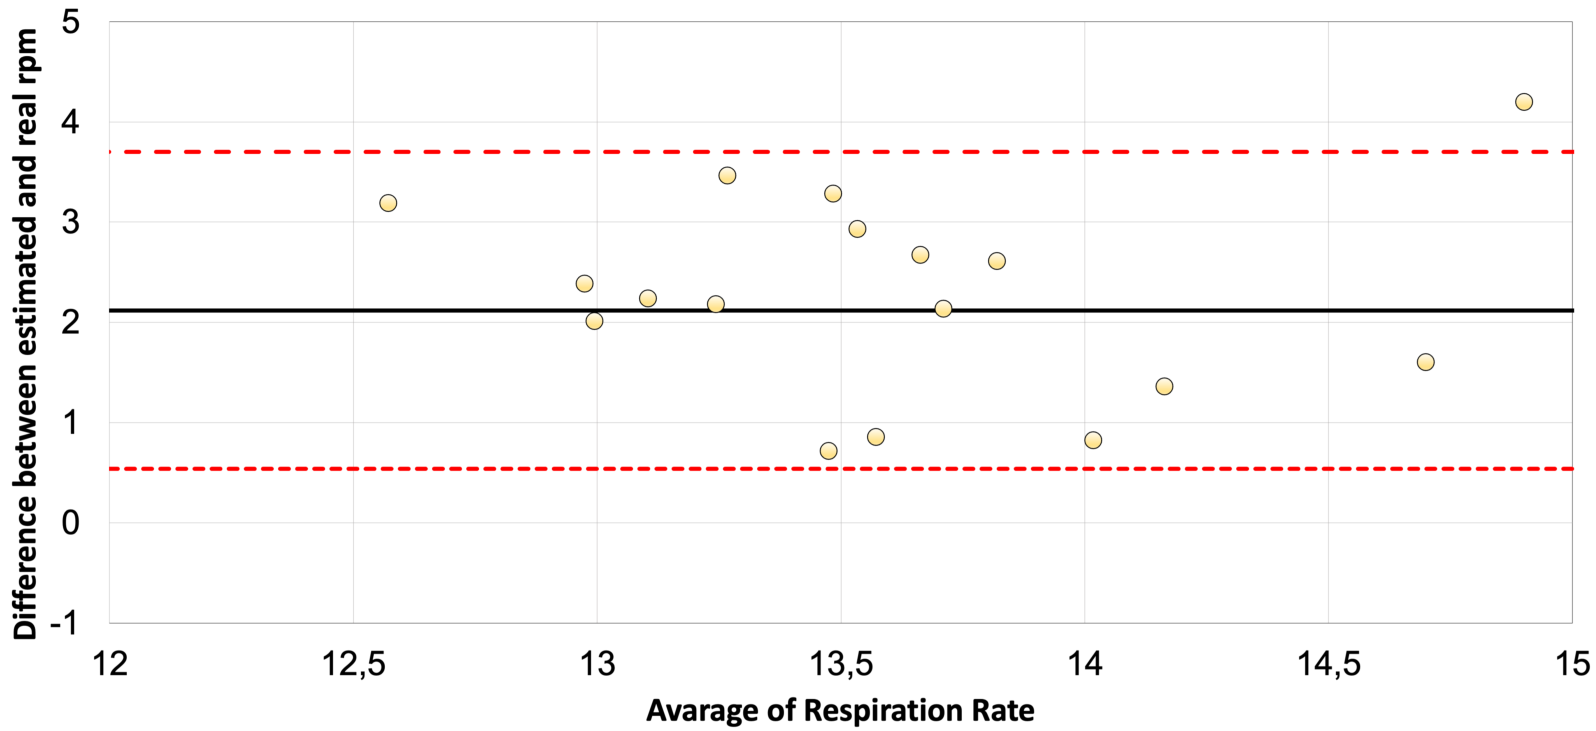
\includegraphics[width=\textwidth]{img/balnd1.pdf}

  \caption{Bland Altman Plot of estimated rpm from the pipeline compared to the value of the ground truth - Normal bed and supine position}
  \label{fig:baln1}
  \vspace{1.5cm}
  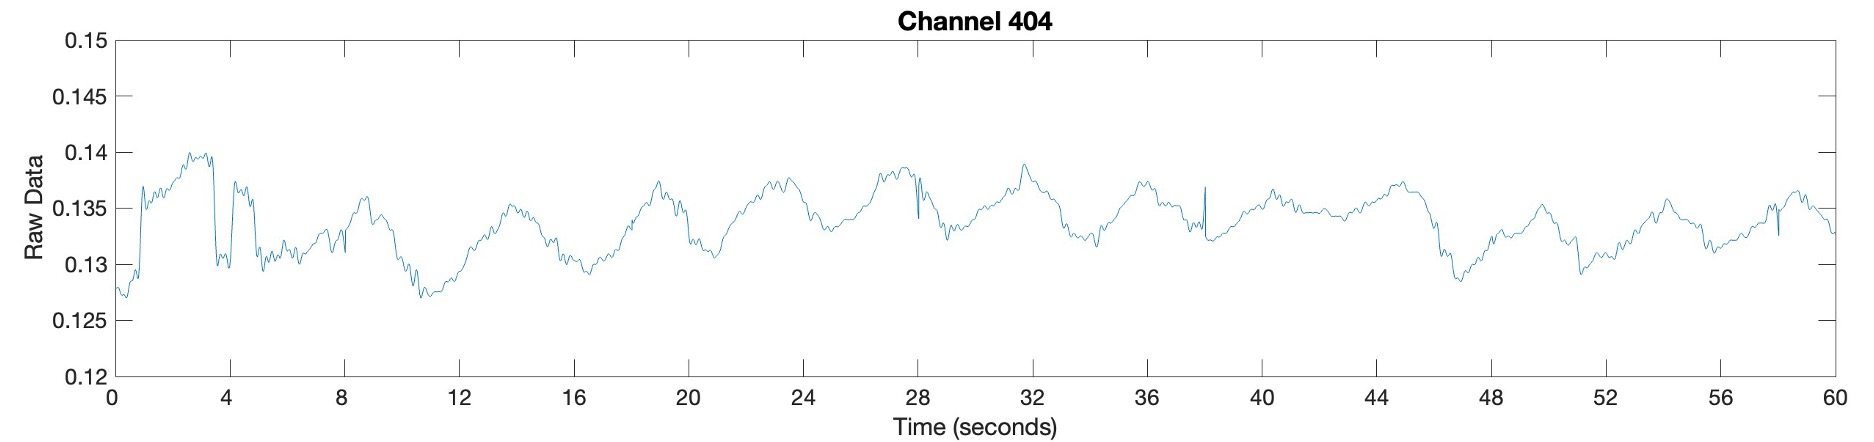
\includegraphics[width=\textwidth]{img/404.jpg}
  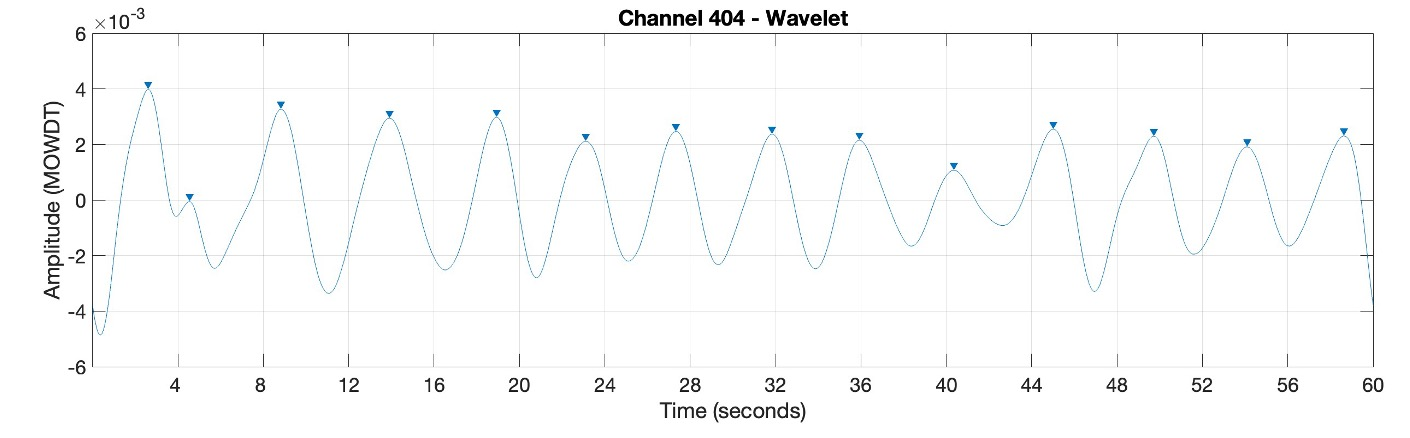
\includegraphics[width=\textwidth]{img/404_wave.jpg}
\caption{Raw data and denoised signal using MODWTMRA of the channel with the highest percentage of confidence (92\%) - Normal bed and supine position}
  \label{fig:rec}
\end{figure}

\clearpage
%%%%%% Rocking BED - Prone %%%%%%
\subsubsection{Result Rocking Bed in Prone Position}  % \label{cap:ResultNormalBed1}

The estimated respiratory rate per minute (rpm) while the participants are in prone position with the mattress placed on a rocking bed is further presented. 

Table \ref{tab:LeftMov} presented the estimated rpm using binary and weighted approach compared with the rpm given by the ground truth. The approaches retrieve an almost identical rpm. 

\vspace{0.5cm}
\begin{table}[h]
    \centering
    \begin{tabular}{|c|c|c|}
 
    \hline 
    Binary & Weighed &RPM (NOXA1) \\ 
    \hline 
16         &    16     &   12.6296 \\ 
15.3684     &   15.3684    &     14.168 \\ 
15.6818    &    15.6818   &     13.2588 \\ 
15.5     &   15.4286    &    13.8107 \\ 
15.8333    &    15.8333    &     13.485 \\ 
16        &     16   &     12.6052 \\ 
16        &     16   &     11.0417 \\ 
15.7059    &    15.7059   &     12.9088 \\ 
15.5333    &    15.5333   &     13.0502 \\ 
16.3333    &    16.3333  &      11.1723 \\ 
14.5625     &   14.5625   &     14.6869 \\ 
15.5294    &    15.5294   &     11.3484 \\ 
14.7273    &    14.7273   &     13.0399 \\ 
14.7778    &    14.7778   &     9.54872 \\ 
15.4444     &   15.4444   &     11.7918 \\ 
14.9286    &    14.9286   &     12.8182 \\ 
15.8333    &    15.8333   &     9.53453 \\ 
14.619     &    14.619    &     9.5416 \\ 
\hline 
\end{tabular}
\caption{Estimated rpm using binary and weighted approach of the pipeline
compared with the rpm given by the ground truth
- Rocking bed and prone position}
\label{tab:ProneMov}

\end{table}


Table \ref{tab:ProneRockingMetrics} present the average rpm for both approaches  
and the relative mean absolute error (MAE) and mean absolute percentage error (MAPE). As just discussed in the previous paragraph there is no substantial difference between the two different approaches. The data on which to focus more is the number of breaths that the algorithm misses, represented by MAE and expressed in percentage by MAPE. The average number is 2.5rpm, which means that if we consider the estimated average of 15.2rpm the error is almost 20\%, which is too high for an approach that must be used in the medical field.

%\vspace{0.5cm}
\begin{table}[h]
    \centering
    \begin{tabular}{|c|c|c|}
    \hline 
    & Binary & Weighed \\ 
    
    \hline 
    rpm mean & 15.4655  & 15.4615  \\
MAE resp   &   3.2326   &  3.2286 \\ 
MAPE resp   & 28.5509   & 28.5221 \\ 
    \hline 
\end{tabular}
\caption{Evarage number of breath for each approach with the relative mean
absolute error (MAE) and mean absolute percentage error (MAE) - Rocking bed
and prone position}
\label{tab:ProneRockingMetrics}
\end{table}

Figure \ref{fig:baln1} show the Bland–Altman plot, presented in section \ref{cap:plottino}, of the estimated rpm from the pipeline compared to the value of the ground truth. It helps to visualize the data from Table \ref{tab:ProneRockingMetrics} in respect of the error. Since the result for the approaches is similar the data presented with this plot refers to the weighted approach only.

Figure \ref{fig:rec} shows the denoised signal using MODWTMRA with the highest accuracy (92\%) for the supine position with a normal mattress.

\begin{figure}[p]
  \centering
  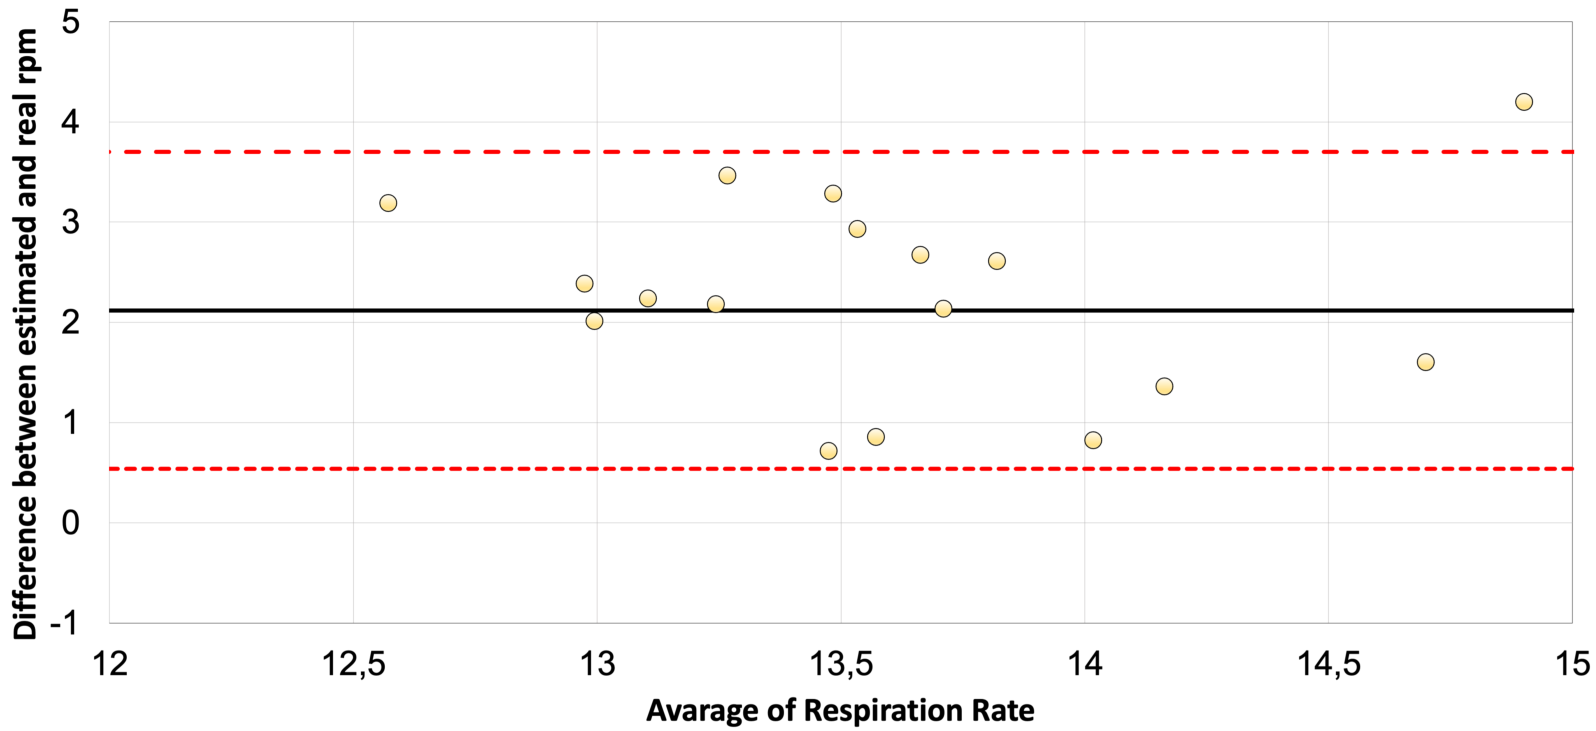
\includegraphics[width=\textwidth]{img/balnd1.pdf}

  \caption{Bland Altman Plot of estimated rpm from the pipeline compared to the value of the ground truth - Normal bed and supine position}
  \label{fig:baln1}
  \vspace{1.5cm}
  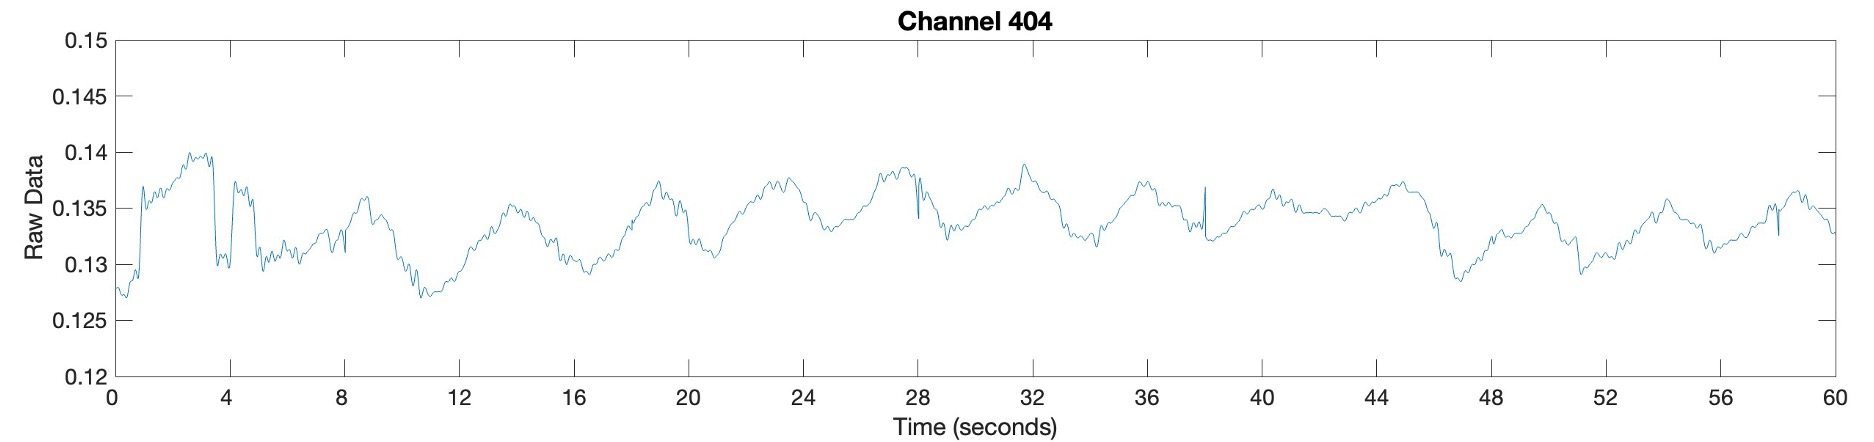
\includegraphics[width=\textwidth]{img/404.jpg}
  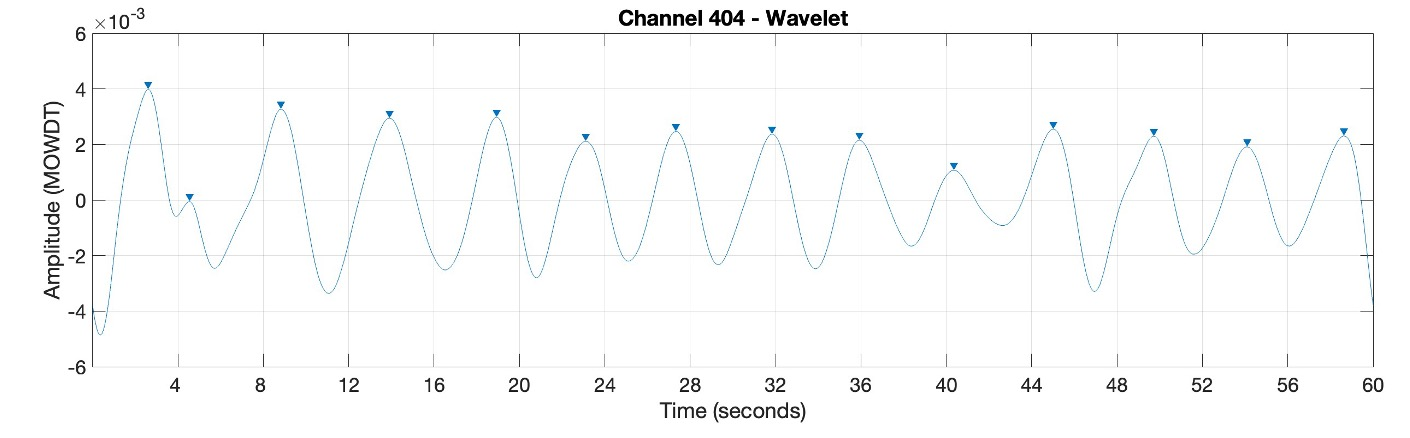
\includegraphics[width=\textwidth]{img/404_wave.jpg}
\caption{Raw data and denoised signal using MODWTMRA of the channel with the highest percentage of confidence (92\%) - Normal bed and supine position}
  \label{fig:rec}
\end{figure}

\clearpage
%%%%%% Rocking BED - RIGHT %%%%%%
\subsubsection{Result Rocking Bed in Right Side }  % \label{cap:ResultNormalBed1}

The estimated respiratory rate per minute (rpm) while the participants are in right side position with the mattress placed on a rocking bed is further presented. 

Table \ref{tab:RightMov} presented the estimated rpm using binary and weighted approach compared with the rpm given by the ground truth. The approaches retrieve an almost identical rpm. 

\vspace{0.5cm}
\begin{table}[h]
    \centering
    \begin{tabular}{|c|c|c|}
 
    \hline 
    Binary & Weighed &RPM (NOXA1) \\ 
    \hline 
15.8095    &  15.8095   &   11.7955 \\ 
15.2105    &     15.1  &    11.9185 \\ 
15.5652    &  15.5652 &     11.8639 \\ 
15.8261    &  15.8261    &    12.28 \\ 
15.6667    &  15.6667   &  12.0136 \\ 
15.1176   &   15.1176   &   12.8838 \\ 
15.3571   &   15.3571  &    11.5695 \\ 
15    &  14.8696   &   12.8922 \\ 
15.1176  &    15.1176  &     11.587 \\ 
15.2857   &   15.2857  &    11.2449 \\ 
15.3333   &   15.3333   &   11.7082 \\ 
15.3684    &    15.35   &   13.9497 \\ 
15.6154    &  15.4286   &   11.6145 \\ 
15.4286    &  15.4286  &    13.9913 \\ 
15.2727    &  15.2727   &   11.6172 \\ 
15.3      &  15.3    &  13.3257 \\ 
15.1667   &   15.1667  &    13.5179 \\ 
14.9231   &   14.9286   &   13.5767 \\ 
\hline 
\end{tabular}
\caption{Estimated rpm using binary and weighted approach of the pipeline
compared with the rpm given by the ground truth - Rocking bed and right side position}
\label{tab:RightMov}

\end{table}

Table \ref{tab:RightMov} present the average rpm for both approaches  
and the relative mean absolute error (MAE) and mean absolute percentage error (MAPE). As just discussed in the previous paragraph there is no substantial difference between the two different approaches. The data on which to focus more is the number of breaths that the algorithm misses, represented by MAE and expressed in percentage by MAPE. The average number is 2.9rpm, which means that if we consider the estimated average of 15.3rpm the error is almost 24\%, which is too high for an approach that must be used in the medical field.

%\vspace{0.5cm}

\begin{table}
    \centering 
    \begin{tabular}{|c|c|c|}
    \hline 
    & Binary & Weighed  \\ 
    
    \hline 
    rpm mean &15.3536  & 15.3291 \\
    MAE resp & 2.9452 &      2.9208 \\ 
    MAPE  & 24.4008 \%& 24.1986\% \\ 
    \hline 
\end{tabular}
\caption{Evarage number of breath for each approach with the relative mean
absolute error (MAE) and mean absolute percentage error (MAE) - Rocking bed
and right side}
\label{tab:RightRockingMetrics}
\end{table}

Figure \ref{fig:baln1} show the Bland–Altman plot, presented in section \ref{cap:plottino}, of the estimated rpm from the pipeline compared to the value of the ground truth. It helps to visualize the data from Table \ref{tab:RightRockingMetrics} in respect of the error. Since the result for the approaches is similar the data presented with this plot refers to the weighted approach only.

Figure \ref{fig:rec} shows the denoised signal using MODWTMRA with the highest accuracy (92\%) for the supine position with a normal mattress.

\begin{figure}[p]
  \centering
  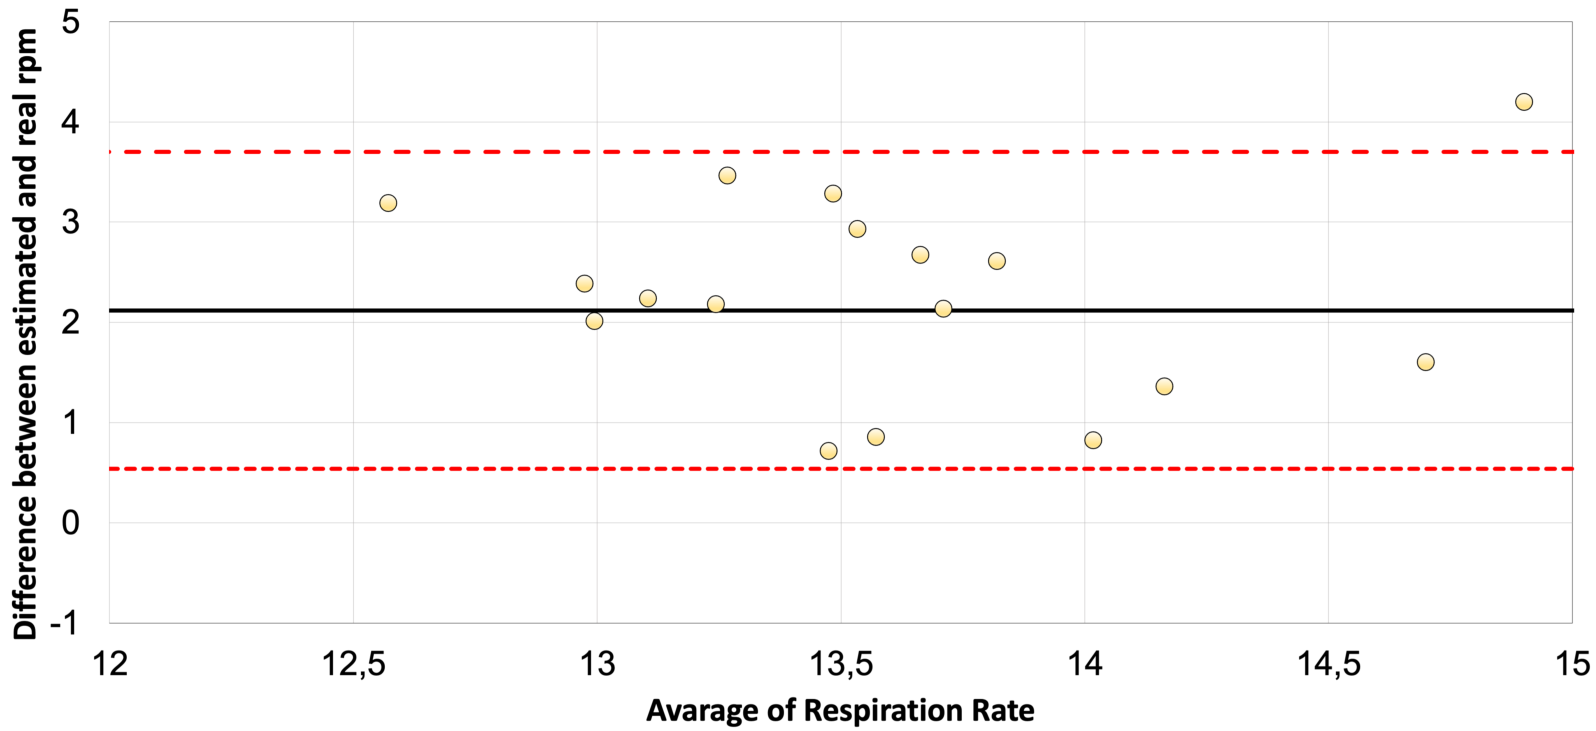
\includegraphics[width=\textwidth]{img/balnd1.pdf}

  \caption{Bland Altman Plot of estimated rpm from the pipeline compared to the value of the ground truth - Normal bed and supine position}
  \label{fig:baln1}
  \vspace{1.5cm}
  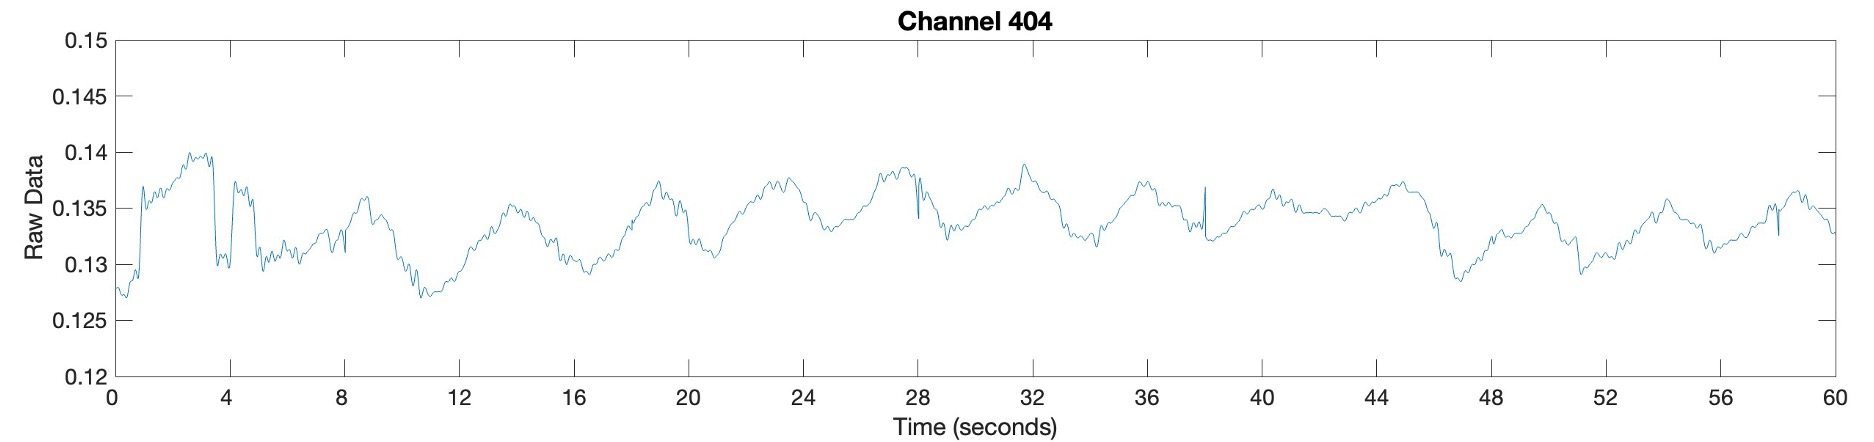
\includegraphics[width=\textwidth]{img/404.jpg}
  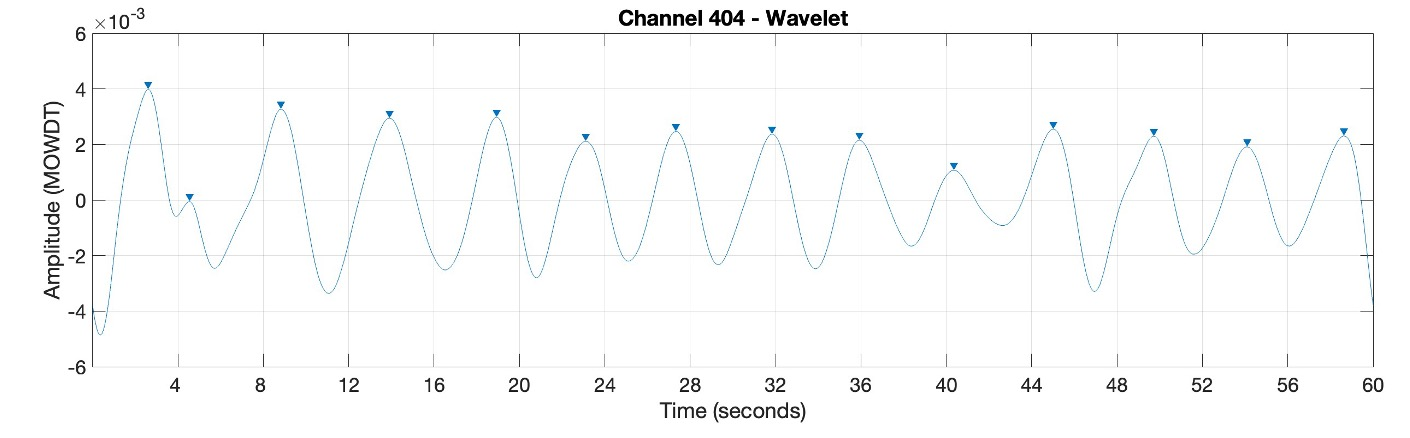
\includegraphics[width=\textwidth]{img/404_wave.jpg}
\caption{Raw data and denoised signal using MODWTMRA of the channel with the highest percentage of confidence (92\%) - Normal bed and supine position}
  \label{fig:rec}
\end{figure}



\section{Result for Savitzky–Golay filter} \label{cap:ResultSG}

The result presented in this section are denoised with Savitzky–Golay filter and are
 divided into normal bed, section \ref{cap:normalSavitz}, and rocking bed \ref{cap:RockSavitx}. Inside both sections are presented the result for each position for the binary and weighted approach.


%%%%%% NORMAL BED %%%%%%
\subsection{Normal Bed} \label{cap:normalSavitz}

The participant in this phase has to perform a series of jumps before lying on the mattress due to recreating the increase or decrease of the breath rate between the different sleep stages. This phase aims to understand the feasibility of extracting breath rate from the mat. For this phase, the mattress is placed on a standard bed.

%%%%%% NORMAL BED - SUPINE %%%%%%

\subsubsection{Result Normal Bed in Supine Position}  
The estimated respiratory rate per minute (rpm) while the participants are supine with the mattress placed on a normal bed is further presented. Table \ref{tab:SupineNormalStillsg} presented the estimated rpm using binary and weighted approach compared with the rpm given by the ground truth. The approaches retrieve an almost identical rpm, this result may be due to the choice of the minimum confidence value at 80\% that allows keeping only the best signal, maybe with higher confidence can be seen a higher difference between the two approaches. 

\vspace{0.5cm}
\begin{table}[h]
    \centering
    \begin{tabular}{|c|c|c|}
 
    \hline 
    Binary & Weighed & RPM (NOXA1) \\ 
    \hline 
    12.8529  & 12.8333  & 13.485  \\ 
    12.0909  & 12.0909  & 13.1443  \\ 
    11.9167  & 11.9167  & 12.5154  \\ 
    13.3333  & 13.4  & 13.117  \\ 
    12.2857  & 12.2857  & 13.6077 \\ 
    12.5833  & 12.3077  & 13.8993 \\ 
    11.6  & 11.6 & 12.0681  \\ 
    9 &  9  & 11.4768  \\ 
    11.1667  & 10.625  & 12.1549  \\ 
    14.5 & 14.5  & 12.8028 \\ 
    14.3333  & 14.3333  & 12.3275  \\ 
    11.625  & 11.625  & 10.9785  \\ 
    13.125  & 13.125  & 11.8441  \\ 
    13.1111  & 13.1111  & 12.6438  \\ 
    13.3077  & 13.3077  & 11.5351  \\ 
    13.6667  & 13.6667  & 11.99  \\ 
    11.5  & 11.5  & 11.9868 \\ 
    11.4545  & 11.2308  & 11.7824 \\ 
    \hline 
\end{tabular}
\caption{Estimated rpm using binary and weighted approach of the pipeline
compared with the rpm given by the ground truth
- Normal bed and supine position}
\label{tab:SupineNormalStillsg}

\end{table}

Table \ref{tab:SupineNormalStillMetricssg} present the average rpm for both approaches  
and the relative mean absolute error (MAE) and mean absolute percentage error (MAPE). As just discussed in the previous paragraph there is no substantial difference between the two different approaches. The data on which to focus more is the number of breaths that the algorithm misses, represented by MAE and expressed in percentage by MAPE. The average number is 2rpm, which means that if we consider the estimated average of 14.5rpm the error is almost 20\%, quite high for an approach that must be used in the medical field.

%\vspace{0.5cm}
\begin{table}[h]
    \centering
    \begin{tabular}{|c|c|c|}
    \hline 
    & Binary SGf & binary Waveleft & weighed  SGf & weighed Waveleft \\ 
    \hline 
    rpm mean &    \\ 
    MAE resp & 1.0796 &       1.1422  \\ 
    MAPE resp & 8.7793 \%  & 9.2789 \% \\ 
    \hline 
    \end{tabular}
    
    \caption{Evarage number of breath for each approach with the relative mean
    absolute error (MAE) and mean absolute percentage error (MAE) - Normal bed
    and supine position}
    \label{tab:SupineNormalStillMetricssg}    
\end{table}
    
    

Figure \ref{fig:baln1} show the Bland–Altman plot, presented in section \ref{cap:plottino}, of the estimated rpm from the pipeline compared to the value of the ground truth. It helps to visualize the data from Table \ref{tab:SupineNormalStillMetricssg} in respect of the error. Since the result for the approaches is similar the data presented with this plot refers to the weighted approach only.

Figure \ref{fig:rec} shows the denoised signal using MODWTMRA with the highest accuracy (92\%) for the supine position with a normal mattress.

\begin{figure}[p]
  \centering
  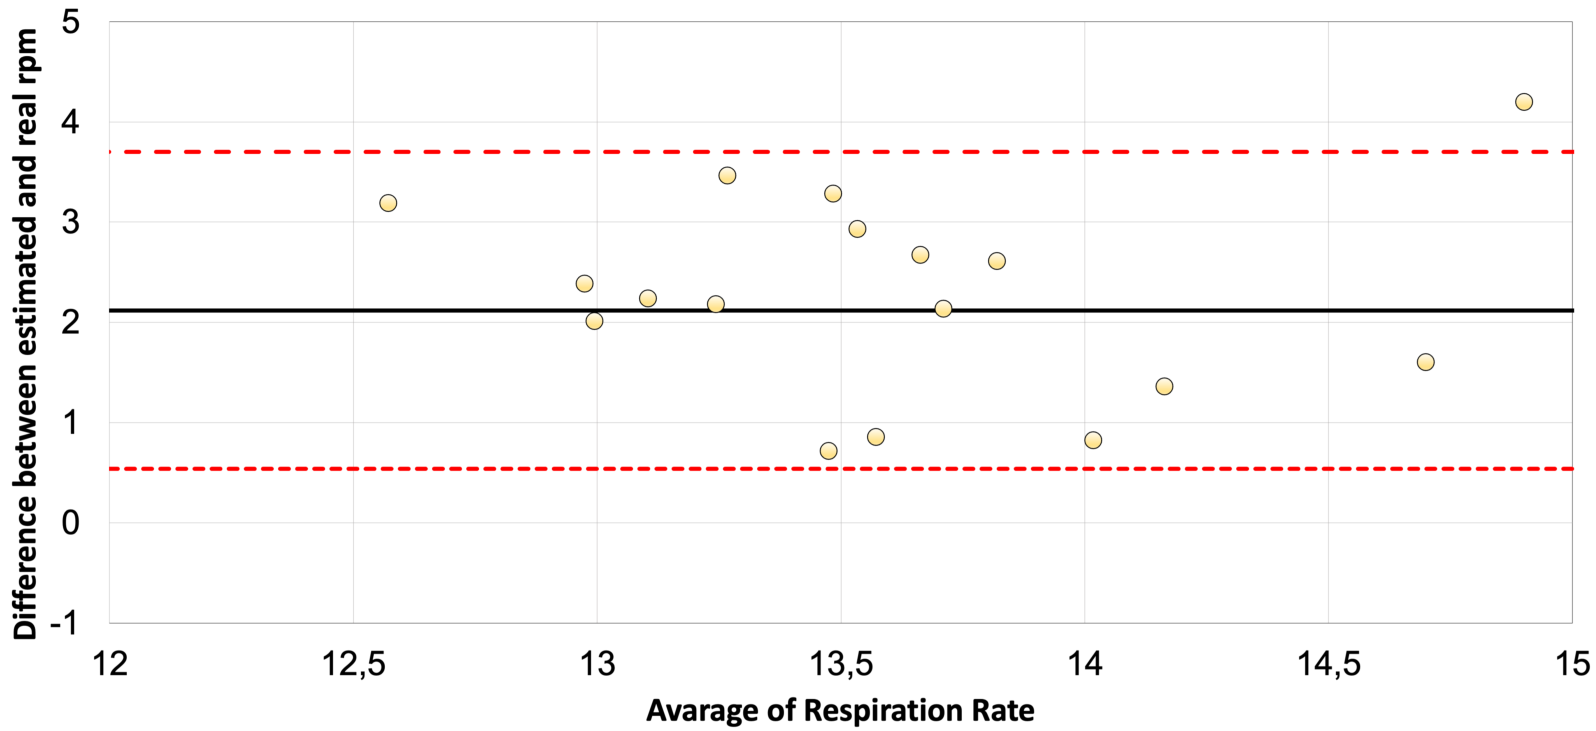
\includegraphics[width=\textwidth]{img/balnd1.pdf}

  \caption{Bland Altman Plot of estimated rpm from the pipeline compared to the value of the ground truth - Normal bed and supine position}
  \label{fig:baln1}
  \vspace{1.5cm}
  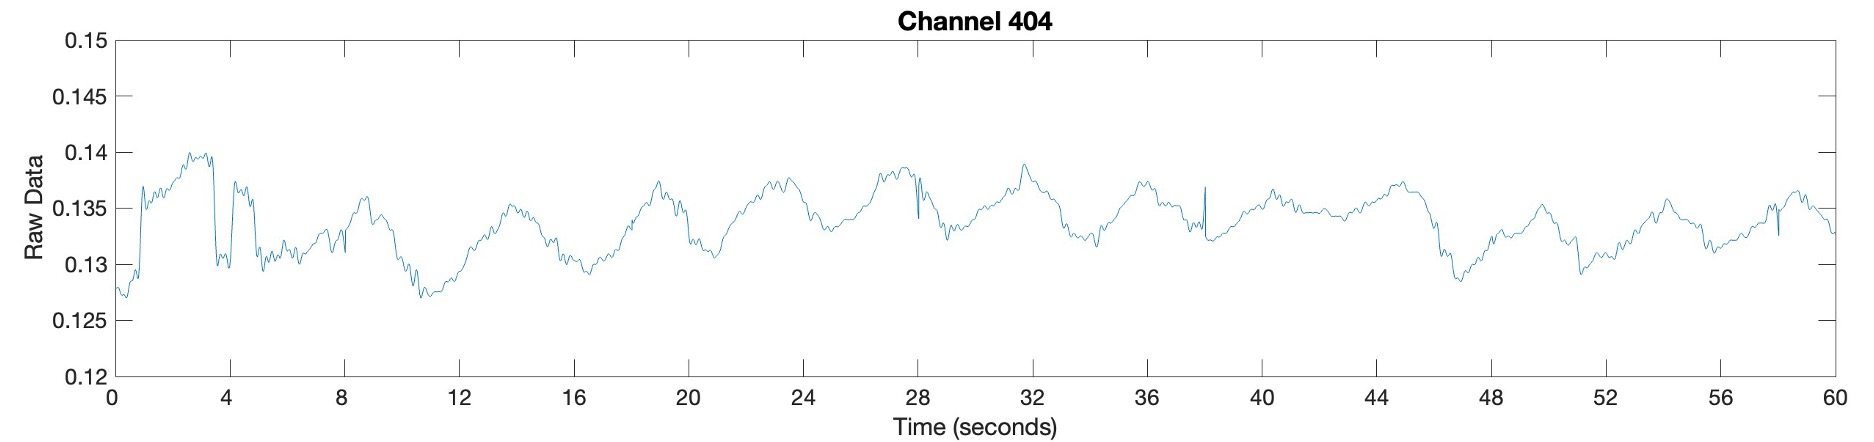
\includegraphics[width=\textwidth]{img/404.jpg}
  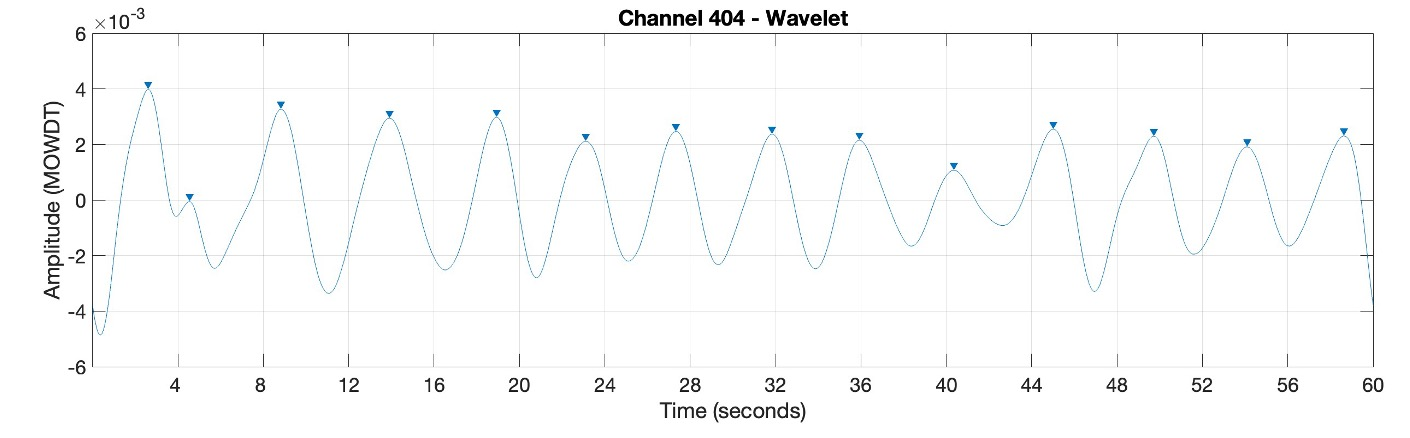
\includegraphics[width=\textwidth]{img/404_wave.jpg}
\caption{Raw data and denoised signal using MODWTMRA of the channel with the highest percentage of confidence (92\%) - Normal bed and supine position}
  \label{fig:rec}
\end{figure}


\clearpage
%%%%%% Rocking  Bed %%%%%%
\subsection{Rocking Bed}\label{cap:RockSavitx}
The second part of the data collection aims to understand if the movement of the
rocking bed could influence the signal. The participant has to lie on the mattress without jumps, to have less variability in the data. For this phase, the mattress is placed on a rocking bed, which periods have been fixed at 4 seconds (15 periods in a minute) with an acceleration of 0.25 $m/s^2$.


%%%%%% Rocking BED - SUPINE %%%%%%

\subsubsection{Result Rocking Bed in Supine Position}  % \label{cap:ResultNormalBed1}

The estimated respiratory rate per minute (rpm) while the participants are supine with the mattress placed on a rocking bed is further presented. 

Table \ref{tab:SupineMovsg} presented the estimated rpm using binary and weighted approach compared with the rpm given by the ground truth. The approaches retrieve an almost identical rpm. 

\vspace{0.5cm}
\begin{table}[h]
    \centering
    \begin{tabular}{|c|c|c|}
 
    \hline 
    Binary & Weighed & RPM (NOXA1) \\ 
    \hline 
14.1667     &  14.1667  &     10.7609 \\ 
14.0667   &    14.0667  &     11.3077 \\ 
13.5     &     13.5  &     13.1449 \\ 
13.75    &     13.75   &    11.3366 \\ 
12.9474    &   12.9474 &      12.7314 \\ 
12.4615   &    12.4615    &   11.8892 \\ 
12.6875   &    12.6875     &    11.42 \\ 
13.5   &    13.6364 &      13.0092 \\ 
14.6154  &     14.6154  &     13.2539 \\ 
13.1429   &    13.1429  &     11.6391 \\ 
14.375   &     14.375  &     12.2165 \\ 
15.4286   &    15.4286   &    11.9216 \\ 
14.6667   &    14.6667   &    11.3091 \\ 
14.8182   &    14.8182   &    13.8905 \\ 
14.5385   &    14.5385  &     11.3344 \\ 
13.9091    &   13.9167  &     11.4474 \\ 
13.8824  &     13.8824  &     11.6675 \\ 
13.8667   &    13.8667   &    13.4799 \\ 
\hline
    \end{tabular}
\caption{Estimated rpm using binary and weighted approach of the pipeline compared with the rpm given by the ground truth - Rocking bed and supine position}
\label{tab:SupineMovsg}

\end{table}

Table \ref{tab:SupineMovsg} present the average rpm for both approaches  
and the relative mean absolute error (MAE) and mean absolute percentage error (MAPE). As just discussed in the previous paragraph there is no substantial difference between the two different approaches. The data on which to focus more is the number of breaths that the algorithm misses, represented by MAE and expressed in percentage by MAPE. The average number is 3rpm, which means that if we consider the estimated average of 15.1rpm the error is almost 25\%, is too high for an approach that must be used in the medical field.

%\vspace{0.5cm}

\begin{table}[h]

    \centering

\begin{tabular}{|c|c|c|c|c|}
\hline 
& Binary & Weighed \\ 
 
\hline 
rpm mean & 13.9068 &  13.9148  \\  
MAE rpm   &  1.8091&      1.8171 \\ 
MAPE   & 15.5385\% &  15.6004\% \\ 

\hline 
\end{tabular}
\caption{Evarage number of breath for each approach with the relative mean
absolute error (MAE) and mean absolute percentage error (MAE) - Rocking bed
and supine position}
\label{tab:SupineRockingMetricssg}
\end{table}

Figure \ref{fig:baln1} show the Bland–Altman plot, presented in section \ref{cap:plottino}, of the estimated rpm from the pipeline compared to the value of the ground truth. It helps to visualize the data from Table \ref{tab:SupineRockingMetricssg} in respect of the error. Since the result for the approaches is similar the data presented with this plot refers to the weighted approach only.

Figure \ref{fig:rec} shows the denoised signal using MODWTMRA with the highest accuracy (92\%) for the supine position with a normal mattress.

\begin{figure}[p]
  \centering
  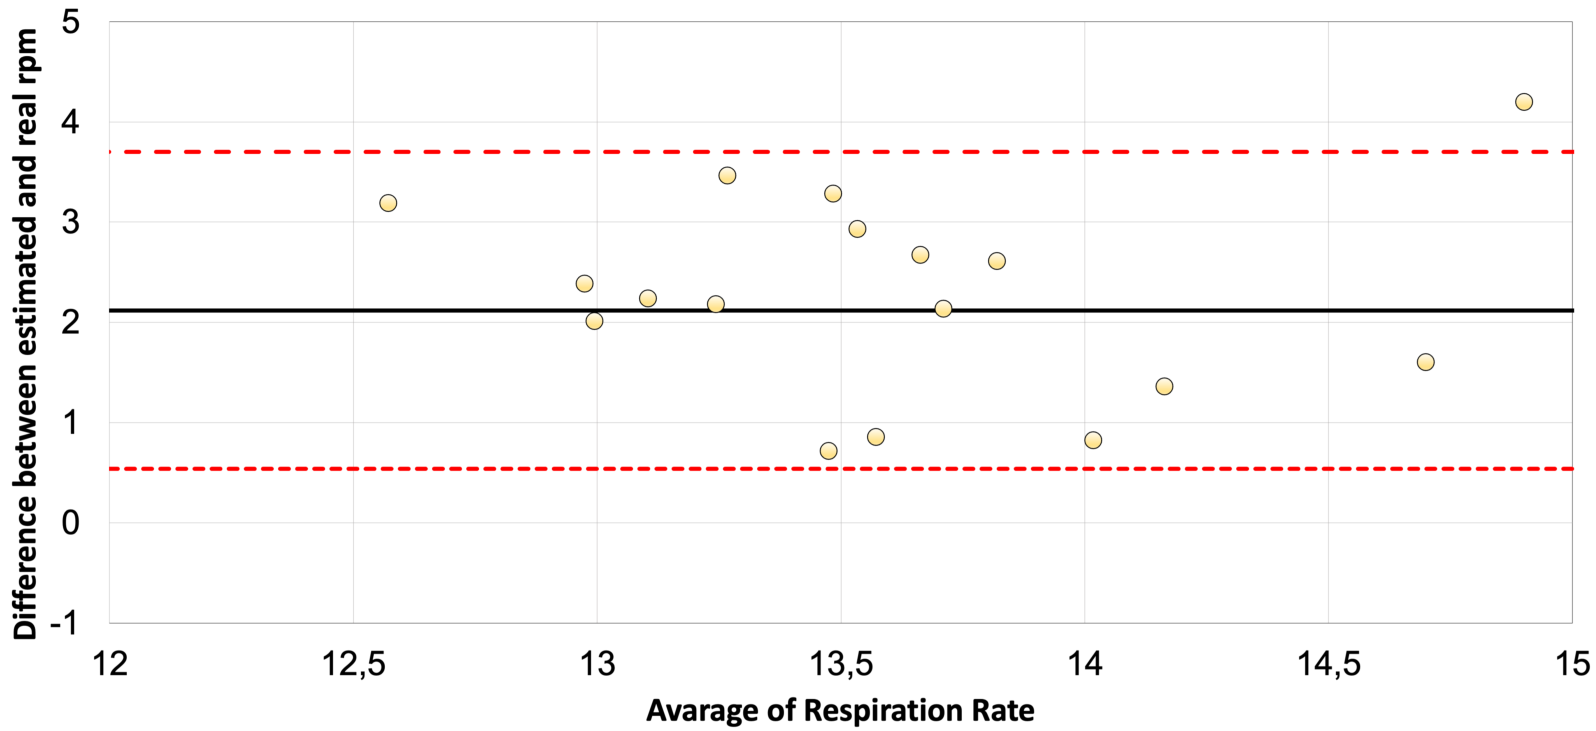
\includegraphics[width=\textwidth]{img/balnd1.pdf}

  \caption{Bland Altman Plot of estimated rpm from the pipeline compared to the value of the ground truth - Rocking bed and supine position}
  \label{fig:baln1}
  \vspace{1.5cm}
  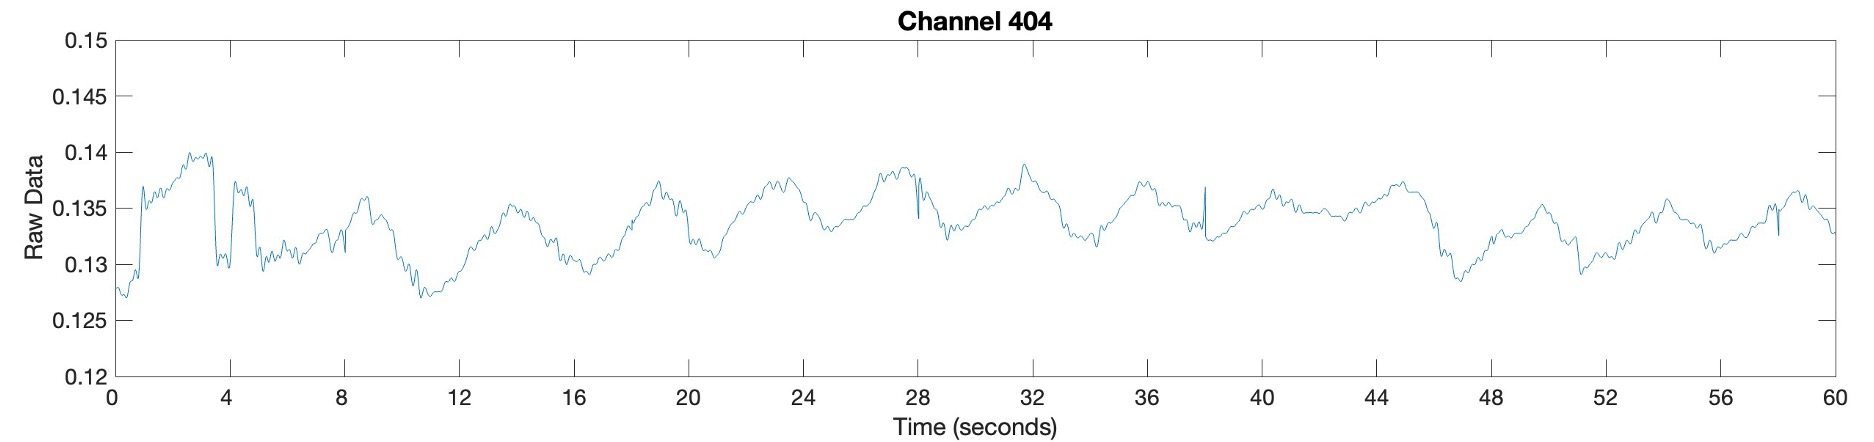
\includegraphics[width=\textwidth]{img/404.jpg}
  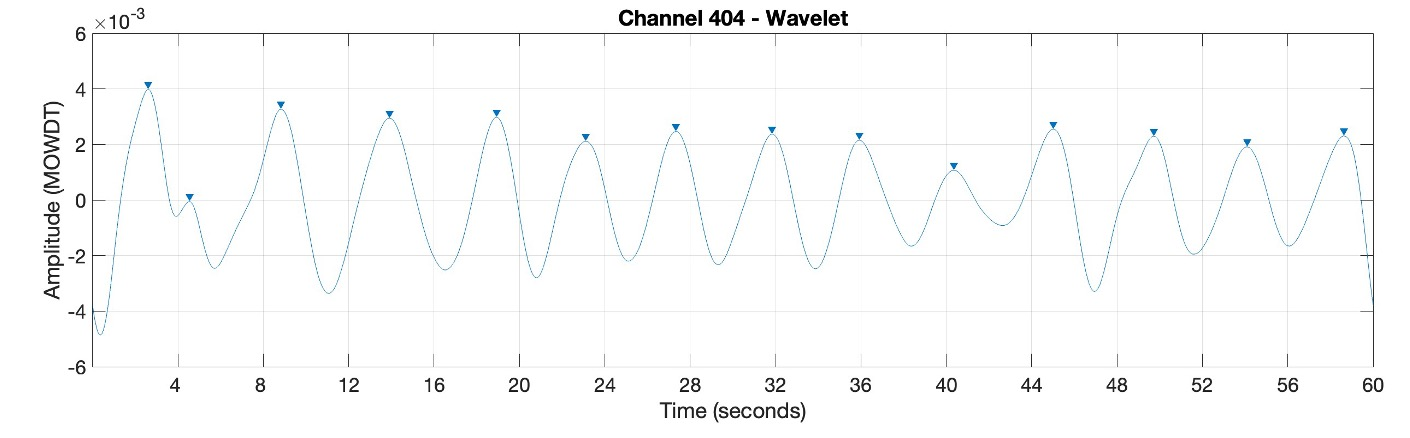
\includegraphics[width=\textwidth]{img/404_wave.jpg}
\caption{Raw data and denoised signal using MODWTMRA of the channel with the highest percentage of confidence (92\%) - Normal bed and supine position}
  \label{fig:rec}
\end{figure}

%%%%%% CONSIDERAZIONI FINALI %%%%%%
\section{Final Remarks on the Results}

This chapter presented the results of the pipeline. Since it has several parameters that can be chosen and they influence the outcome, they are commented on.

%\subsection{Evaluation of the approaches}
The pipeline allows choosing which approach to use to denoise the signal, in order to be able to give it as input to a peak finder. The different approaches are Multiresolution Overlap Discrete Wavelet Transform (described in Chapter \ref{Wavelet}) and Savitzky–Golay filter (described in Chapter \ref{sg}).
Both approaches are used in the context of the estimation of respiratory rate \cite{Sadek2017NonintrusiveStudy, Chen2008UnconstrainedSleep}, for this reason, it has been very important to have the possibility to compare them to understand which one could perform better in the context of this thesis.

The result presented in the previous section highlighted how the Savitzky–Golay filter has a lower error in respect of the wavelet approach. In fact, focusing on the MAPE it is 10\% lower in most of the positions and in both settings. The average error is 1 breath in respect of MODWTMRA which arrive up to 4 in the case of a prone position with a rocking bed.


%\subsection{Evaluation of the settings}

One of the aims of the data collection conducted during this study, described in Chapter \ref{cap:dataCollection}, has been to understand if the movement of the rocking bed could influence the signal from the mattress.
Even if the bed is designed to have an inaudible rocking mechanism, it is reasonable to expect that the movement could influence the data acquisition. The raw data visually present more noise, but the denoise approaches are able to exclude it and estimate the respiratory rate.
This can be seen in the reconstruction of the data, as shown in figure [PLACEHOLDER], and also in the result of the metrics that have a slight increase of the error but not higher as expected.
From the respiratory rate point of view, the influence on the error is mostly given by the chosen approach rather than the bed set. 

The position of the participant on the bed also seems to be decisive, in the prone position the error increases particularly and in the supine has the minimum error. It may depend on the movement of the chest that in the prone position changes.\\


\begin{comment}

%\begin{table}[h]
    \centering
    \begin{tabular}{|c|c|c|c|}
    \hline 
    Binary SGf & binary Waveleft & weighed  SGf & weighed Waveleft  \\%resp rate & toolbox \\ 
    \hline 
    12.8529 & 14.8438 & 12.8333 & 14.7353 \\ %& 13.485 & 14 \\ %
    12.0909 & 14 & 12.0909 & 14  \\ % & 13.1443 & 13 \\ 
    11.9167 & 15.125 & 11.9167 & 15.125 \\ %& 12.5154 & 13 \\ 
    13.3333 & 13.8333 & 13.4 & 13.8333 \\ %& 13.117 & 13 \\ 
    12.2857 & 14.4286 & 12.2857 & 14.4286 \\ %& 13.6077 & 14 \\ 
    12.5833 & 15.5 & 12.3077 & 15.5 \\ %& 13.8993& 15 \\ 
    11.6 & 15 & 11.6 & 15 \\ %& 12.0681 & 15 \\ 
    9 & 11 & 9 & 11 \\ %& 11.4768 & 15 \\ 
    11.1667 & 14.3333 & 10.625 & 14.3333 \\ %& 12.1549 & 14 \\ 
    14.5 & 17 & 14.5 & 17 \\ %& 12.8028 & 13 \\ 
    14.3333 & 15 & 14.3333 & 15 \\ %& 12.3275 & 14 \\ 
    11.625 & 14.1667 & 11.625 & 14.1667 \\ %& 10.9785 & 11 \\ 
    13.125 & 15.125 & 13.125 & 15.125 \\ %& 11.8441 & 11 \\ 
    13.1111 & 14.7778 & 13.1111 & 14.7778 \\ %& 12.6438 & 10 \\ 
    13.3077 & 15 & 13.3077 & 15 \\ %& 11.5351 & 11 \\ 
    13.6667 & 14 & 13.6667 & 14 \\ %& 11.99 & 10 \\ 
    11.5 & 14.2222 & 11.5 & 14.2222 \\ %& 11.9868 & 10 \\ 
    11.4545 & 14.1667 & 11.2308 & 13.8571 \\ %& 11.7824 & 10 \\ 
    \hline 
    \end{tabular}
    \caption{Breath per minute for each approach, results from Noxtural
    - A back position on a normal mattress}
\end{table}


\begin{table}[h]
\centering
\begin{tabular}{|c|c|c|c|c|}
\hline 
& Binary SGf & binary Waveleft & weighed  SGf & weighed Waveleft \\ 
\hline 
RMSE resp & 
    1.2517  &  2.4000  &  1.3043  &  2.3806 \\ 
RMSE tool &      2.4481  &  2.9583   & 2.4960  &  2.9332 \\ 
MAE resp & 1.0796 &   2.1731 &     1.1422 &  2.1499 \\ 
MAE tool &     2.0256 & 2.4179 & 2.0633 &  2.3947 \\ 
MAPE resp & 8.7793 & 17.8104 & 9.2789 & 17.6198 \\ 
MAPE tool & 16.3648 & 21.3416 & 16.5938 & 21.1266 \\ 
\hline 
\end{tabular}

\caption{Metrics to evaluate the participant in back position with still mattress}
\end{table}




\subsubsection{Back position with moving mattress}
\begin{table}[h]
\centering
\begin{tabular}{|c|c|c|c|}
\hline 
Binary SGf & binary Waveleft & weighed  SGf & weighed Waveleft  \\% & resp rate & toolbox \\ 
\hline 
14.1667 & 15.5 & 14.1667 & 15.5 \\% & 10.7609 & 8 \\ 
14.0667 & 16.1333 & 14.0667 & 16.1333 \\% & 11.3077 & 6 \\ 
13.5 & 15.3333 & 13.5 & 15.3333 \\% & 13.1449 & 8 \\ 
13.75 & 14.9474 & 13.75 & 14.9474 \\% & 11.3366 & 8 \\ 
12.9474 & 15.1 & 12.9474 & 15.1 \\% & 12.7314 & 6 \\ 
12.4615 & 15.6364 & 12.4615 & 15.6364 \\% & 11.8892 & 9 \\ 
12.6875 & 14.6923 & 12.6875 & 14.6923 \\% & 11.42 & 9 \\ 
13.5 & 15.2222 & 13.6364 & 15.2222 \\% & 13.0092 & 10 \\ 
14.6154 & 15.1667 & 14.6154 & 15.1667 \\% & 13.2539 & 12 \\ 
13.1429 & 14.6667 & 13.1429 & 14.6667 \\% & 11.6391 & 11 \\ 
14.375 & 15 & 14.375 & 15 \\% & 12.2165 & 11 \\ 
15.4286 & 14.75 & 15.4286 & 14.75 \\% & 11.9216 & 12 \\ 
14.6667 & 15 & 14.6667 & 15 \\% & 11.3091 & 13 \\ 
14.8182 & 14.625 & 14.8182 & 14.625 \\% & 13.8905 & 12 \\ 
14.5385 & 15.6154 & 14.5385 & 15.6154 \\% & 11.3344 & 13 \\ 
13.9091 & 15 & 13.9167 & 14.8182 \\% & 11.4474 & 11 \\ 
13.8824 & 15.1765 & 13.8824 & 15.1765 \\% & 11.6675 & 11 \\ 
13.8667 & 14.6154 & 13.8667 & 14.6154 \\% & 13.4799 & 12 \\ 
\hline 
\end{tabular}


\caption{Breath per minutes for each approach, result from Noxtural and toolbox  - Back position moving mattress}

\end{table}


\begin{table}[h]

    \centering

\begin{tabular}{|c|c|c|c|c|}
\hline 
& Binary SGf & binary Waveleft & weighed  SGf & weighed Waveleft \\ 
 
\hline 
RMSE resp &  2.1340  &  3.2155  &  2.1365  &  3.2047 \\ 
RMSE tool &     4.2192  &  5.5405  &  4.2259   & 5.5334 \\  
MAE resp & 1.8091 &   3.0234 &     1.8171 &  3.0133 \\ 
MAE tool &     3.7957 & 5.0100 & 3.8037 &  4.9999 \\  
MAPE resp & 15.5385 & 25.7324 & 15.6004 & 25.6442 \\ 
MAPE tool & 44.4027 & 58.5849 & 44.4823 & 58.4931 \\ 

\hline 
\end{tabular}

\caption{Metrics to evaluate the participant in back position with moving mattress}
\end{table}


\subsubsection{Left position with still mattress}
\begin{table}\begin{tabular}{|llllll|}
\hline 
Binary SGf & binary Waveleft & weighed  SGf & weighed Waveleft & resp rate & toolbox \\ 
\hline 
13.375 & 14.6364 & 13.375 & 14.6364 & 11.2045 & 10 \\ 
13.6667 & 15 & 13.6667 & 15 & 12.7397 & 11 \\ 
14 & 16 & 13.5 & 15.25 & 13.0613 & 12 \\ 
14.3571 & 14.2 & 14.3571 & 14.2 & 12.2669 & 12 \\ 
14 & 19 & 14 & 19 & 12.1628 & 13 \\ 
12.8 & 15 & 12.6667 & 14.5 & 13.6039 & 13 \\ 
11.8 & 14.2222 & 11.8 & 14.2222 & 13.1398 & 13 \\ 
14 & 15.6667 & 14 & 15.6667 & 11.5445 & 14 \\ 
13.8333 & 14.7 & 13.8333 & 14.7 & 10.77 & 11 \\ 
13.8889 & 15.8571 & 13.8889 & 15.8571 & 14.2216 & 12 \\ 
13.0833 & 15.5556 & 13.0833 & 15.5556 & 13.1656 & 12 \\ 
14.1111 & 16.5714 & 13.7 & 16.5714 & 12.9764 & 12 \\ 
14.2 & 15 & 14.2 & 15 & 10.9055 & 13 \\ 
13.25 & 15.125 & 13.25 & 15.125 & 13.2294 & 11 \\ 
12.7692 & 15.7143 & 12.2857 & 15.5 & 12.8524 & 11 \\ 
13.9167 & 15.2 & 13.6154 & 15.2 & 11.3824 & 13 \\ 
13 & 14.6 & 13 & 14.6 & 13.5579 & 11 \\ 
13 & 15.8889 & 13 & 15.8889 & 11.6069 & 12 \\ 
\hline 
\end{tabular}
\caption{Breath per minutes for each approach, result from Noxtural and toolbox
- Left position still mattress}
\end{table}

\begin{table}
\begin{tabular}{|lllll|}
\hline 
& Binary SGf & binary Waveleft & weighed  SGf & weighed Waveleft \\ 

\hline 
RMSE resp &
      1.7158  &  3.2950  &  1.6774  &  3.2425 \\
RMSE  tool &    1.8743  &  3.6582   & 1.7959   & 3.5879 \\
MAE resp & 1.3922 &   2.4545 &     1.3591 &  2.8934 \\ 
MAE tool &     1.6584 & 2.9748 & 1.5716 &  3.3596 \\
MAPE resp & 11.8278 & 24.62 & 11.5556 & 24.0041 \\ 
MAPE tool & 14.4565 & 29.3635 & 13.7188 & 28.6943 \\ 
\hline 
\end{tabular}

\caption{Metrics to evaluate the participant in left position with still mattress}
\end{table}


%\section{Left position with moving mattress}
\begin{table}
\begin{tabular}{|llllll|}
\hline 
Binary SGf & binary Waveleft & weighed  SGf & weighed Waveleft & resp rate & toolbox \\ 
\hline 
13.6875 & 15.0625 & 13.6875 & 15.0625 & 13.6613 & 11 \\ 
14.5294 & 15.5556 & 14.5294 & 15.5556 & 11.4545 & 8 \\ 
14.5 & 15.8824 & 14.5 & 15.8824 & 12.3288 & 6 \\ 
13.9444 & 16.1176 & 13.9444 & 16.1176 & 10.8865 & 7 \\ 
14.0455 & 15.2083 & 14.0455 & 15.2083 & 11.4082 & 9 \\ 
13.44 & 15.3214 & 13.4231 & 15.3103 & 12.2589 & 6 \\ 
13.9091 & 15.4583 & 13.9091 & 15.4583 & 13.7093 & 8 \\ 
14 & 15.4375 & 14 & 15.4375 & 12.7019 & 10 \\ 
14.4 & 15.2353 & 14.4 & 15.2353 & 13.3305 & 12 \\ 
14.5769 & 15.5556 & 14.5769 & 15.5556 & 13.7078 & 13 \\ 
14.7 & 15.2143 & 14.7 & 15.2143 & 13.5674 & 14 \\ 
14.8421 & 15.2 & 14.8421 & 15.1538 & 11.8694 & 15 \\ 
14.85 & 15.5556 & 14.85 & 15.5556 & 13.4086 & 15 \\ 
15.5 & 14.75 & 15.5 & 14.75 & 13.9781 & 15 \\ 
13.6667 & 14.5 & 13.6667 & 14.5 & 12.4749 & 13 \\ 
13.8571 & 15.25 & 13.8571 & 15.25 & 12.4049 & 13 \\ 
13.375 & 14.625 & 13.7 & 14.7273 & 13.4108 & 12 \\ 
13.75 & 14.2857 & 14.1667 & 14.3333 & 13.4716 & 14 \\ 
\hline 
\end{tabular}
\caption{Breath per minutes for each approach, result from Noxtural and toolbox
- Left position moving mattress}
\end{table}

\begin{table}

\begin{tabular}{|lllll|}
\hline 
& Binary SGf & binary Waveleft & weighed  SGf & weighed Waveleft \\ 

\hline 
RMSE resp &
      1.7259  &  2.7236  &  1.7331   & 2.7232 \\
RMSE  tool &   4.1782  &  5.2608  &  4.1829   & 5.2627 \\
MAE resp & 1.4229 &   2.4545 &     1.4592 &  2.4597 \\ 
MAE tool &     3.0939 & 4.0953 & 3.1063 &  4.1004 \\
MAPE resp & 11.6751 & 19.9605 & 11.9443 & 19.9959 \\ 
MAPE tool & 39.3516 & 50.7242 & 39.4533 & 50.7631 \\ 
\hline 
\end{tabular}

\caption{Metrics to evaluate the participant in left position with moving mattress}
\end{table}



%\section{Belly position with still mattress}
\begin{table}
\begin{tabular}{|llllll|}
\hline 
Binary SGf & binary Waveleft & weighed  SGf & weighed Waveleft & resp rate & toolbox \\ 
\hline 
15.3 & 15.7 & 15.3 & 15.7 & 11.5949 & 14 \\ 
14.8125 & 15.7333 & 14.8125 & 15.7333 & 11.1628 & 16 \\ 
14.2 & 16.1 & 14.2 & 16.1 & 11.0005 & 16 \\ 
14.8889 & 15.6667 & 14.8889 & 15.6667 & 10.4762 & 15 \\ 
13.5 & 15.25 & 13.5 & 15.25 & 10.4723 & 15 \\ 
13.8571 & 14.5714 & 13.8571 & 14.5714 & 9.5345 & 14 \\ 
13.8571 & 15.5714 & 13.8571 & 15.5714 & 9.5467 & 13 \\ 
14.3 & 15.875 & 14.3 & 15.875 & 13.5758 & 14 \\ 
15 & 14 & 15 & 14 & 11.1779 & 14 \\ 
13.9 & 14.375 & 13.9 & 14.375 & 9.5345 & 14 \\ 
13.8667 & 14.4667 & 13.8667 & 14.4667 & 9.5841 & 15 \\ 
13.8235 & 14.5 & 13.8235 & 14.5 & 11.8196 & 14 \\ 
14.0714 & 14.2143 & 14.0714 & 14.2143 & 11.8153 & 10 \\ 
13 & 13.9474 & 13 & 13.9474 & 9.5223 & 8 \\ 
14.4828 & 15.037 & 14.4828 & 15.037 & 10.8508 & 8 \\ 
14.3793 & 14.931 & 14.3793 & 14.931 & 10.8876 & 7 \\ 
13.7 & 15.25 & 13.7 & 15.25 & 10.9705 & 7 \\ 
14.1818 & 15.3333 & 14.1818 & 15.3333 & 11.237 & 6 \\ 
\hline 
\end{tabular}

\caption{Breath per minutes for each approach, result from Noxtural and toolbox
- Belly position still mattress}
\end{table}


\begin{table}
\begin{tabular}{|lllll|}
\hline 
& Binary SGf & binary Waveleft & weighed  SGf & weighed Waveleft \\ 

\hline 
RMSE resp &
     3.4835  &  4.3281 &   3.4835  &  4.3281 \\
RMSE  tool & 3.8127   & 4.3162   & 3.8127  &  4.3162 \\
MAE resp & 3.3532 &   4.2088 &     3.3532 &  4.2088 \\ 
MAE tool &     2.6347 & 2.8957 & 2.6347 &  2.8957 \\
MAPE resp & 31.914 & 39.9076 & 31.914 & 39.9076 \\ 
MAPE tool & 32.6041 & 36.5982 & 32.6041 & 36.5982 \\ 
\hline 
\end{tabular}

\caption{Metrics to evaluate the participant in belly position with moving mattress}
\end{table}


%\section{Belly position with moving mattress}
\begin{table}
\begin{tabular}{|llllll|}
\hline 
Binary SGf & binary Waveleft & weighed  SGf & weighed Waveleft & resp rate & toolbox \\ 
\hline 
14.6667 & 16 & 14.6667 & 16 & 12.6296 & 9 \\ 
14.0455 & 15.3684 & 14.0455 & 15.3684 & 14.168 & 12 \\ 
14.3478 & 15.6818 & 14.3478 & 15.6818 & 13.2588 & 13 \\ 
14.381 & 15.5 & 14.3636 & 15.4286 & 13.8107 & 13 \\ 
13.7143 & 15.8333 & 13.7143 & 15.8333 & 13.485 & 13 \\ 
14 & 16 & 14 & 16 & 12.6052 & 14 \\ 
16.1 & 16 & 16.1 & 16 & 11.0417 & 17 \\ 
15.7647 & 15.7059 & 15.7647 & 15.7059 & 12.9088 & 17 \\ 
14.7333 & 15.5333 & 14.7333 & 15.5333 & 13.0502 & 16 \\ 
14.6 & 16.3333 & 14.6 & 16.3333 & 11.1723 & 17 \\ 
14.3846 & 14.5625 & 14.3846 & 14.5625 & 14.6869 & 16 \\ 
13.8889 & 15.5294 & 13.8889 & 15.5294 & 11.3484 & 13 \\ 
13.7273 & 14.7273 & 13.7273 & 14.7273 & 13.0399 & 11 \\ 
13.8235 & 14.7778 & 13.8235 & 14.7778 & 9.5487 & 10 \\ 
13.6111 & 15.4444 & 13.6111 & 15.4444 & 11.7918 & 11 \\ 
13.2667 & 14.9286 & 13.2667 & 14.9286 & 12.8182 & 8 \\ 
12.9375 & 15.8333 & 12.9375 & 15.8333 & 9.5345 & 8 \\ 
13.3 & 14.619 & 13.3 & 14.619 & 9.5416 & 13 \\ 
\hline 
\end{tabular}\caption{Breath per minutes for each approach, result from Noxtural and toolbox
- Belly position moving mattress}
\end{table}

\begin{table}
\begin{tabular}{|lllll|}
\hline 
& Binary SGf & binary Waveleft & weighed  SGf & weighed Waveleft \\ 
 
\hline 
RMSE resp &
    2.4778  &  3.6110  &  2.4775  &  3.6092 \\
RMSE  tool &  2.7357  &  3.8447  &  2.7352  &  3.8422 \\
MAE resp & 1.9835 &   3.2326 &     1.9825 &  3.2286 \\ 
MAE tool &     2.1737 & 3.2326 & 2.1728 &  3.1687 \\ 
MAPE resp & 17.8949 & 28.5509 & 17.8879 & 28.5221 \\ 
MAPE tool & 20.8138 & 30.5337 & 20.8064 & 30.5032 \\ 
\hline 
\end{tabular}

\caption{Metrics to evaluate the participant in belly position with moving mattress}
\end{table}



%\section{Right position with still mattress}
\begin{table}\begin{tabular}{|llllll|}
\hline 
Binary SGf & binary Waveleft & weighed  SGf & weighed Waveleft & resp rate & toolbox \\ 

\hline 
14.5714 & 16.1667 & 14.5714 & 16.1667 & 12.4771 & 17 \\ 
14 & 17.75 & 14 & 17.75 & 13.0835 & 17 \\ 
16.5 & 16.5 & 16.5 & 16.5 & 14.3858 & 17 \\ 
14.7778 & 15.25 & 14.7778 & 15.25 & 12.7261 & 17 \\ 
14.5 & 15.8333 & 14.5 & 15.8333 & 13.4867 & 17 \\ 
13.9333 & 15 & 13.9333 & 15 & 12.9816 & 16 \\ 
15 & 15.2353 & 15 & 15.2353 & 14.0566 & 15 \\ 
13.7692 & 15.1667 & 13.7692 & 15.1667 & 12.038 & 16 \\ 
14 & 15.5 & 14 & 15.5 & 11.4923 & 12 \\ 
14.6 & 13 & 14.6 & 13 & 11.9625 & 10 \\ 
15 & 13.3333 & 14.3333 & 13.5 & 11.0151 & 9 \\ 
16.5 & 15.5 & 16.5 & 15.5 & 11.9016 & 10 \\ 
14.5 & 14.3333 & 14.5 & 14.3333 & 11.4255 & 10 \\ 
12.2857 & 13.8333 & 12.2857 & 13.8333 & 12.5227 & 7 \\ 
12.8333 & 15.2 & 12.8333 & 15.2 & 11.5945 & 10 \\ 
12.3333 & 14.0909 & 12.3333 & 14.0909 & 13.4141 & 8 \\ 
12.3636 & 14.5 & 12.4783 & 14.4286 & 13.5282 & 11 \\ 
13.4286 & 15.2308 & 12.875 & 15.2308 & 12.9839 & 11 \\ 
\hline 
\end{tabular}
\caption{Breath per minutes for each approach, result from Noxtural and toolbox
- Right position still mattress}
\end{table}
\begin{table}\begin{tabular}{|lllll|}
\hline 
& Binary SGf & binary Waveleft & weighed  SGf & weighed Waveleft \\ 
\hline 
RMSE resp &
     2.1572  &  2.7087  &  2.0877  &  2.7156 \\
RMSE  tool &    3.5099  &   3.6341   & 3.4330 &   3.6416 \\
MAE resp & 1.8214 &   2.4638 &     1.7593 &  2.4691 \\ 
MAE tool &     3.0440 & 2.9772 & 2.9826 &  2.9825 \\
MAPE resp & 14.9336 & 19.9146 & 14.4066 & 19.9693 \\ 
MAPE tool & 28.9627 & 30.229 & 28.3295 & 30.2958 \\ 
\hline 
\end{tabular}

\caption{Metrics to evaluate the participant in right position with still mattress}
\end{table}


%\section{Right position with moving mattress}
\begin{table}\begin{tabular}{|llllll|}
\hline 
Binary SGf & binary Waveleft & weighed  SGf & weighed Waveleft & resp rate & toolbox \\ 
\hline 
14.2273 & 15.8095 & 14.2273 & 15.8095 & 11.7955 & 10 \\ 
13.625 & 15.2105 & 13.5294 & 15.1 & 11.9185 & 9 \\ 
13.9524 & 15.5652 & 13.9524 & 15.5652 & 11.8639 & 8 \\ 
15 & 15.8261 & 14.7826 & 15.8261 & 12.28 & 10 \\ 
14.5652 & 15.6667 & 14.375 & 15.6667 & 12.0136 & 10 \\ 
13.625 & 15.1176 & 13.625 & 15.1176 & 12.8838 & 10 \\ 
14.4118 & 15.3571 & 14.4118 & 15.3571 & 11.5695 & 12 \\ 
14.72 & 15 & 14.72 & 14.8696 & 12.8922 & 13 \\ 
14.85 & 15.1176 & 14.85 & 15.1176 & 11.587 & 14 \\ 
15 & 15.2857 & 15 & 15.2857 & 11.2449 & 14 \\ 
15.2917 & 15.3333 & 15.28 & 15.3333 & 11.7082 & 15 \\ 
15.5294 & 15.3684 & 15.5 & 15.35 & 13.9497 & 15 \\ 
14.5625 & 15.6154 & 14.5294 & 15.4286 & 11.6145 & 16 \\ 
14.8182 & 15.4286 & 14.8182 & 15.4286 & 13.9913 & 16 \\ 
14.7333 & 15.2727 & 14.7333 & 15.2727 & 11.6172 & 16 \\ 
14.8824 & 15.3 & 14.8824 & 15.3 & 13.3257 & 16 \\ 
14.75 & 15.1667 & 14.75 & 15.1667 & 13.5179 & 16 \\ 
15.0667 & 14.9231 & 15.0667 & 14.9286 & 13.5767 & 16 \\ 
\hline 
\end{tabular}
\caption{Breath per minutes for each approach, result from Noxtural and toolbox
- Right position moving mattress}
\end{table}

\begin{table}\begin{tabular}{|lllll|}
\hline 
& Binary SGf & binary Waveleft & weighed  SGf & weighed Waveleft \\ 

\hline 
RMSE resp &
     2.4083   & 3.1106  &  2.3763 &   3.0860 \\
RMSE  tool &    2.9182  &  3.6785   & 2.8737  &  3.6656 \\
MAE resp & 2.2367 &   2.9452 &     2.2046 &  2.9208 \\ 
MAE tool &     2.3325 & 2.7195 & 2.3041 &  2.7152 \\
MAPE resp & 18.5442 & 24.4008 & 18.2803 & 24.1986 \\ 
MAPE tool & 22.0502 & 26.6562 & 21.761 & 26.5883 \\ 
\hline 
\end{tabular}

\caption{Metrics to evaluate the participant in right position with moving mattress}
\end{table}

\end{comment}